\documentclass[10pt]{article}

\usepackage{ifpdf}
\usepackage{booktabs}
\usepackage{array}
\usepackage{paralist}
\usepackage{subfigure}
\usepackage[pdftex]{graphicx}
\usepackage{epstopdf}
\usepackage[cmex10]{amsmath}
\interdisplaylinepenalty=2500
\usepackage{geometry}
\usepackage{multicol}
\geometry{left=1in,right=1in,top=1in,bottom=1in,letterpaper}
\usepackage{fancyhdr}
\pagestyle{fancy}
\renewcommand{\headrulewidth}{0pt}
\lhead{}\chead{}\rhead{}
\lfoot{}\cfoot{\thepage}\rfoot{}

\usepackage{amsfonts}
\usepackage{amstext}
\usepackage{booktabs}
\usepackage{threeparttable}
\usepackage{longtable}
\usepackage{listings}
\usepackage[font=normalsize]{caption}
\usepackage{textcomp}
\usepackage[usenames]{color}
\usepackage{soul}
\usepackage{fancyvrb}
\usepackage{relsize}
\usepackage[noadjust]{cite}
\usepackage{xr-hyper}
\usepackage[usenames,dvipsnames,svgnames,table]{xcolor}
\usepackage[colorlinks=true,linkcolor=black,urlcolor=blue,hyperfootnotes=false,citecolor=LimeGreen]{hyperref}
\usepackage{upquote}
\usepackage[title,titletoc]{appendix}

\usepackage[nottoc,notlof,notlot]{tocbibind}
%\renewcommand{\FancyVerbFormatLine}[1]{\makebox[2mm][l]{}#1}
%\DefineVerbatimEnvironment%
%  {Code}{Verbatim}
%  {fontsize=\relsize{-1.5},
%  samepage=true,
%  frame=single}

\renewcommand{\FancyVerbFormatLine}[1]{\makebox[2mm][l]{}#1}
\DefineVerbatimEnvironment%
  {Notice}{Verbatim}
  {fontsize=\relsize{-1.5},
  samepage=true,
  xleftmargin=15mm,
  framesep=5mm,
  frame=single}

\newcommand{\covemda}{CoVEMDA}
\newcommand{\covemdagithuburl}{https://github.com/tamu-engineering-research/COVID-EMDA}
\newcommand{\matlab}{\textsc{MATLAB}}
\newcommand{\covver}{1.0}
\newcommand{\EILAB}{{\sc EILAB}}
\newcommand{\eilab}{{Energy Intelligence Laboratory (\EILAB{})}}


\definecolor{BackgroundColor}{HTML}{e7f2fa}
\definecolor{SepColor}{HTML}{6ab0de}
\definecolor{DarkGreen}{rgb}{0.0,0.4,0.0}

\usepackage{tikz}
\usetikzlibrary{calc}
\usepackage[framemethod=tikz]{mdframed}
\usepackage{lipsum}


%Command Window
\definecolor{DarkBlue}{RGB}{0,64,115} 
\mdfdefinestyle{commandline}%
{leftmargin=5pt, rightmargin=10pt, innerleftmargin=15pt, 
 middlelinecolor=DarkBlue, 
 middlelinewidth=2pt, 
 frametitlerule=false,
 backgroundcolor=white, 
 frametitle={Command Window}, 
 frametitlefont={\small\sffamily\color{white}\hspace{-1em}}, 
 frametitlebackgroundcolor=DarkBlue, 
 singleextra={\draw[black!15,line width=12pt] 
        ($(O)+(7pt,1pt)$) -- 
        ($(O|-P)+(7pt,-\mdfframetitleboxtotalheight)-(0,1pt)$); 
        \node[inner sep=0pt,color=black]at ($(O)+(7pt,9pt)$)% 
        {$\scriptstyle f\!x$}; }, 
 nobreak, 
}
\lstnewenvironment{Command} {%
    \lstset{
        language=Matlab,
        basicstyle=\small\ttfamily,
        commentstyle=\color{DarkGreen},
        breaklines=true,
        aboveskip=0pt,belowskip=0pt%
        }}
    {}
\surroundwithmdframed[style=commandline]{Command}

\mdfdefinestyle{sourcecode}%
{leftmargin=5pt, rightmargin=10pt, innerleftmargin=15pt, 
 middlelinecolor=DarkBlue, 
 middlelinewidth=2pt, 
 frametitlerule=false,
 backgroundcolor=white, 
 frametitle={Function Definition}, 
 frametitlefont={\small\sffamily\color{white}\hspace{-1em}}, 
 frametitlebackgroundcolor=DarkBlue, 
 singleextra={\draw[black!15,line width=12pt] 
        ($(O)+(7pt,1pt)$) -- 
        ($(O|-P)+(7pt,-\mdfframetitleboxtotalheight)-(0,1pt)$); }, 
 nobreak, 
}
\lstnewenvironment{Code} {%
    \lstset{
        language=Matlab,
        basicstyle=\small\ttfamily,
        commentstyle=\color{DarkGreen},
        stringstyle=\color{purple},
        keywordstyle=\bfseries\color{blue},
        breaklines=true,
        aboveskip=0pt,belowskip=0pt%
        }}
    {}
\surroundwithmdframed[style=sourcecode]{Code}

        
\def\sectionautorefname{Chapter}
\def\subsectionautorefname{Section}
\def\subsubsectionautorefname{Section}
\newcommand{\secref}[1]{\autoref{#1} \nameref{#1}}

\numberwithin{equation}{section}
\numberwithin{table}{section}
\renewcommand{\thetable}{\thesection\mbox{-}\arabic{table}}
\numberwithin{figure}{section}
\renewcommand{\thefigure}{\thesection\mbox{-}\arabic{figure}}



%%% title setting
\title{User's Manual for\\\textbf{\covemda{} Toolbox}}
\author{}
\date{\today}



%%% BEGIN DOCUMENT
\begin{document}
\makeatletter
    \begin{titlepage}
        \begin{center}
            
\includegraphics[width=.7\textwidth]{figures/covemda_logo.png}
            
\includegraphics[width=.3\textwidth]{figures/covid_emda_logo.JPG}%
            \vskip 0.5ex%
            {\huge \@title \par}%
            \vskip 2em%
            {\LARGE Version \covver{} \par}%
            \vskip 1.5em%
            {\large \@date \par}%
            
\vfill
            
\includegraphics[width=.5\textwidth]{figures/ei-lab.png}\\
{\scriptsize
\copyright~2020--2021~\eilab{}\\
All Rights Reserved}
        \end{center}
    \end{titlepage}
\makeatother
\thispagestyle{empty}
\newpage
\tableofcontents
\thispagestyle{empty}


%-------------------------------
\newpage
\setcounter{page}{1}
\section*{Website}
\addcontentsline{toc}{section}{Website}

\vskip 3em
\begin{center}
\url{https://github.com/tamu-engineering-research/COVID-EMDA}
\end{center}
\vskip 5em

This manual is accompanied by the above website. The website refers to the GitHub Repository of COVID-EMDA+ Datahub and \covemda{} Toolbox. The Repository provides the released dataset, the source code of toolbox and a series of supplementary materials -- which should be useful to readers.

%-------------------------------
\newpage
\section{Introduction} \label{sec:intro}

\subsection{Background}

With high contagiousness and long incubation period\cite{who2021}, the COVID-19 pandemic has not only endangered the human life and health, but also seriously affected the economy worldwide. Considering that the operation of power system has been greatly threatened by the pandemic\cite{gillingham2020short}\cite{zhong2020implications}\cite{elavarasan2020covid}, Tsinghua University and Texas A\&M University developed the COVID-EMDA+ Dataset, to track and measure the impact of COVID-19 on the electricity sector.

It was believed that the analysis on the cross-domain data might provided great assistance and support for relevant research concerning the policy development on public health emergencies. On the other hand, it has been increasingly urgent for researchers to explore the actual influences of human interventions like Demand Response (DR) on large-scale power system. From this aspect, changes in residential electricity consumption during the COVID-19 constructed a unique case-study on the correlations among various factors in complex power system\cite{ruan2020cross}\cite{ruan2021quantitative}.

Therefore, a more comprehensive MATLAB toolbox named CoVEMDA was motivated for analysis. Based on COVID-EMDA+ Dataset, CoVEMDA is designed for functionalities including \textbf{Data Visualization}, \textbf{Baseline Estimation} and \textbf{Regression Analysis}, as well as other useful supplementary functions.
\subsection{Features}
\begin{itemize}
    \item[$\bullet$] Data Source. \covemda{} is initially developed to support COVID-EMDA+ Dataset. COVID-EMDA+ cross-domain dataset involves electricity market data, public health data, weather data and mobility data for \textbf{all the existing U.S. electricity marketplaces} and some typical cities\footnote{Which refers to Los Angeles, Boston, New York City, Philadelphia, Chicago, Kansas City, Houston} in these markets. The data released is under strict quality control. To be note, the external data is acceptable for \covemda{}\footnote{This feature should be useful for users with poor connections with official COVID-EMDA+ on GitHub Repository}.
    
    \item[$\bullet$] Baseline Estimation. To get the benchmark against which the impact of COVID-19 is quantified, electricity consumption without the pandemic should be estimated first. Conventional methods for baseline estimation including date and week alignment are introduced in \covemda{}. Meanwhile an \textbf{Ensemble Backcast Model} is carefully designed for more accurate result.
    
    \item[$\bullet$] Regression Analysis. To explore the mechanism underneath the impact of pandemic, several potential influencing factors, namely, public health, social distancing, and commercial activity, are investigated. In account for the multi-dimensional relationship complexity and the variance temporal dynamics presented by those factors, several city-specific restricted vector autoregression models are calibrated in \covemda{}.
    
    \item[$\bullet$] Data Visualization. \covemda{} provides implementation of data visualization under various typical usage scenarios. This includes graphically presenting the changes in generation share of each electricity market over time, displaying the daily electricity demand distribution curve, etc. This feature is designed to be simple and convenient, while keeping the code easy to modify.
    
\end{itemize}

\newpage
\subsection{Support Team}

Together with COVID-EMDA dataset, this project is a collaboration of group members under the supervision of Prof. Le Xie at Texas A\&M University and Prof. Haiwang Zhong at Tsinghua University. The support team keeps processing, correcting and updating the data every day.

\begin{figure}[!ht]
    \centering
    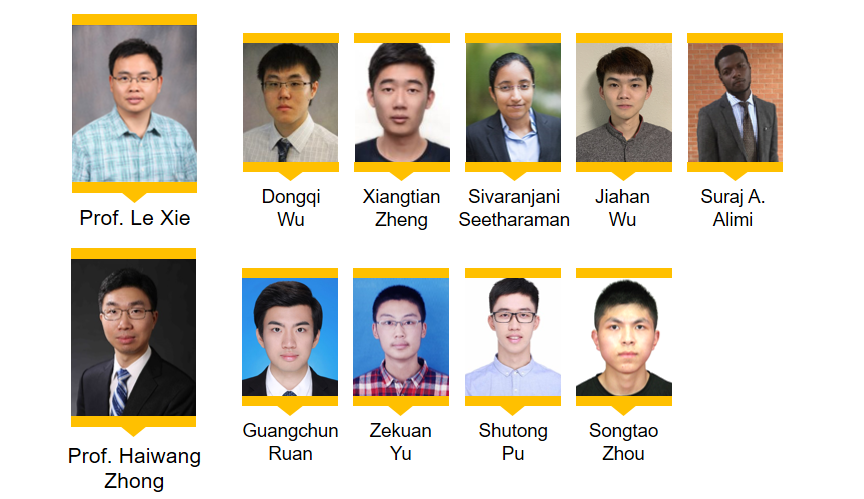
\includegraphics[width=.8\textwidth]{figures/contributor-extend-20210408.png}
    \caption{Support Team}
\end{figure}


\clearpage
\subsection{Suggested Citation}
Publications originated from the employment of data files in COVID-EMDA+, or the supplementary toolbox, please cite the following paper explicitly and properly: 

\begin{itemize}
\item This paper conducts a comprehensive introduction of this data hub and further analysis results for electricity demand across the U.S. The full text is available at: 
\href{https://www.cell.com/joule/pdfExtended/S2542-4351(20)30398-6}{Joule}
and \href{https://arxiv.org/abs/2005.06631}{arXiv}.
\begin{quotation}\footnotesize
G. Ruan, D. Wu, X. Zheng, H. Zhong, C. Kang, M. A. Dahleh, S. Sivaranjani, and L. Xie, ``A Cross-Domain Approach to Analyzing the Short-Run Impact of COVID-19 on the U.S. Electricity Sector,'' Joule, 2020, 4(11), 2322-2337.
\end{quotation}

\item Other research studies of our group are recommended to be cited as:
\begin{itemize}

\item This paper substantiates the pandemic's impacts from the perspectives of power system security, electric power generation, electric power demand and electricity prices. The full text is available at: \href{http://www.enerarxiv.org/page/thesis.html?id=2196}{EnerarXiv}.
\begin{quotation}\footnotesize
G. Ruan, J. Wu, H. Zhong, Q. Xia, and L. Xie, ``Quantitative Assessment of U.S. Bulk Power Systems and Market Operations during the COVID-19 Pandemic,'' 2020. (Submitted to Applied Energy)
\end{quotation}

\item This paper provides a review of the global impacts that COVID-19 has caused on the electricity sector. The full text is available at: \href{https://ieeexplore.ieee.org/abstract/document/9160443}{JPES}.

\begin{quotation}\footnotesize
H. Zhong, Z. Tan, Y. He, L. Xie, and C. Kang, ``Implications of COVID-19 for the Electricity Industry: A Comprehensive Review'', CSEE Journal of Power and Energy Systems, 2020.
\end{quotation}

\end{itemize}

\item This paper introduces the \covemda{} toolbox.
\begin{quotation}
Open-Access Data and Toolbox for Power Sector Analysis During COVID-19.
\end{quotation}



\end{itemize}
\subsection{License}
The code of \covemda~is licensed under the \textbf{MIT License}, and the full text can be found at  \url{https://github.com/tamu-engineering-research/COVID-EMDA/blob/master/LICENSE}, shown as follows.
\begin{Notice}
Copyright (c) 2020 Guangchun Ruan

Permission is hereby granted, free of charge, to any person obtaining a copy
of this software and associated documentation files (the "Software"), to deal
in the Software without restriction, including without limitation the rights
to use, copy, modify, merge, publish, distribute, sublicense, and/or sell
copies of the Software, and to permit persons to whom the Software is
furnished to do so, subject to the following conditions:

The above copyright notice and this permission notice shall be included in all
copies or substantial portions of the Software.

THE SOFTWARE IS PROVIDED "AS IS", WITHOUT WARRANTY OF ANY KIND, EXPRESS OR
IMPLIED, INCLUDING BUT NOT LIMITED TO THE WARRANTIES OF MERCHANTABILITY,
FITNESS FOR A PARTICULAR PURPOSE AND NONINFRINGEMENT. IN NO EVENT SHALL THE
AUTHORS OR COPYRIGHT HOLDERS BE LIABLE FOR ANY CLAIM, DAMAGES OR OTHER
LIABILITY, WHETHER IN AN ACTION OF CONTRACT, TORT OR OTHERWISE, ARISING FROM,
OUT OF OR IN CONNECTION WITH THE SOFTWARE OR THE USE OR OTHER DEALINGS IN THE
SOFTWARE.
\end{Notice}






%-------------------------------
\newpage
\section{Getting Started} \label{sec:start}

\subsection{System Requirements}
To use \covemda~Toolbox you will need:
\begin{itemize}
    \item MATLAB\textsuperscript{\tiny \textregistered} version 9.8 (R2020a)
    \item Deep Learning Toolbox\textsuperscript{\tiny TM} version 14.0
    \item Statistics and Machine Learning Toolbox\textsuperscript{\tiny TM} version 11.7
    \item Financial Toolbox\textsuperscript{\tiny TM} version 5.15
    \item Econometrics Toolbox\textsuperscript{\tiny TM} version 5.5
\end{itemize}

As for the hardware requirements, please refer to the System Requirements of MATLAB according to the specific version\footnote{\url{https://www.mathworks.com/support/requirements/previous-releases.html}}.

\subsection{Data and Toolbox Retrieving}
Both COVID-EMDA dataset and \covemda{} toolbox are available on the GitHub repository. You can either download the whole package of a specific distribution, or subscribe the daily-updated data via cloning the repository to your local folder.

\subsubsection{Download Zip}
    To retrieve \covemda{}, please download the compressed zip-file of GitHub repository.
\begin{itemize}
    \item[$\bullet$] Go to \href{\covemdagithuburl}{\covemda~GitHub repository}.
    \item[$\bullet$] Click the green \textbf{Code} button.
    \item[$\bullet$] Click the \textbf{Download ZIP} button.
    \item[$\bullet$] Uncompress the zip file to certain directory.
\end{itemize}



\subsubsection{Clone GitHub Repository}
To be note, this option required \href{https://git-scm.com/}{Git}/\href{https://desktop.github.com/}{GitHub Desktop} are needed.
    \begin{itemize}
        \item \textbf{Git} required. Open the \textbf{Git Bash} at certain file folder (the one you want the software to be placed in) and type the following command:
\begin{quotation}
\verb!git clone https://github.com/tamu-engineering-research/COVID-EMDA.git!
\end{quotation}
        \item \textbf{GitHub Desktop} required. 
\begin{itemize}
    \item  Go to \href{\covemdagithuburl}{\covemda~GitHub repository}.
    \item Click the green \textbf{Code} button.
    \item Click the \textbf{Open With GitHub Desktop} button.
\end{itemize}
    \end{itemize} 

\clearpage
\subsection{Illustrative Examples}

\subsubsection{Baseline Estimation with Ensemble Backcast Model}\label{subsec:eg_baseline}

\covemda{} provides an efficient tool for load baseline estimation: ensemble backcast model. The corresponding function \verb!cal_baseline! and \verb!plot_baseline! enables the user to calculate and visualize the electricity consumption level without the impact of the pandemic. See Section~\ref{sec:baseline} for more information.

For example, to calculate the baseline of NYISO, the user may enter: (command output omitted)

\begin{Command}
>> t=cal_baseline('nyiso')

t =

  5x2 table

    quantile        result    
    ________    ______________

       0.1      {151x25 table}
      0.25      {151x25 table}
       0.5      {151x25 table}
      0.75      {151x25 table}
       0.9      {151x25 table}
\end{Command}

Access data for q=0.5:

\begin{Command}
>> t.result{3}

ans =

  151x25 table

       date       00:00    01:00    02:00    ...    22:00    23:00
    __________    _____    _____    _____    ...    _____    _____

    2020-02-01    15416    14908    14592    ...    16605    15727
    2020-02-02    15304    14793    14456    ...    16608    15735
    ...
    2020-06-30    16119    15376    14959    ...    18524    17146
\end{Command}

If the user needs to visualize the baseline: (command output omitted)

\begin{Command}
>> plot_baseline('nyiso','Method','backcast');
\end{Command}

The result is displayed in Figure~\ref{fig:backcast_eg}.

\begin{figure}
  \centering
  \noindent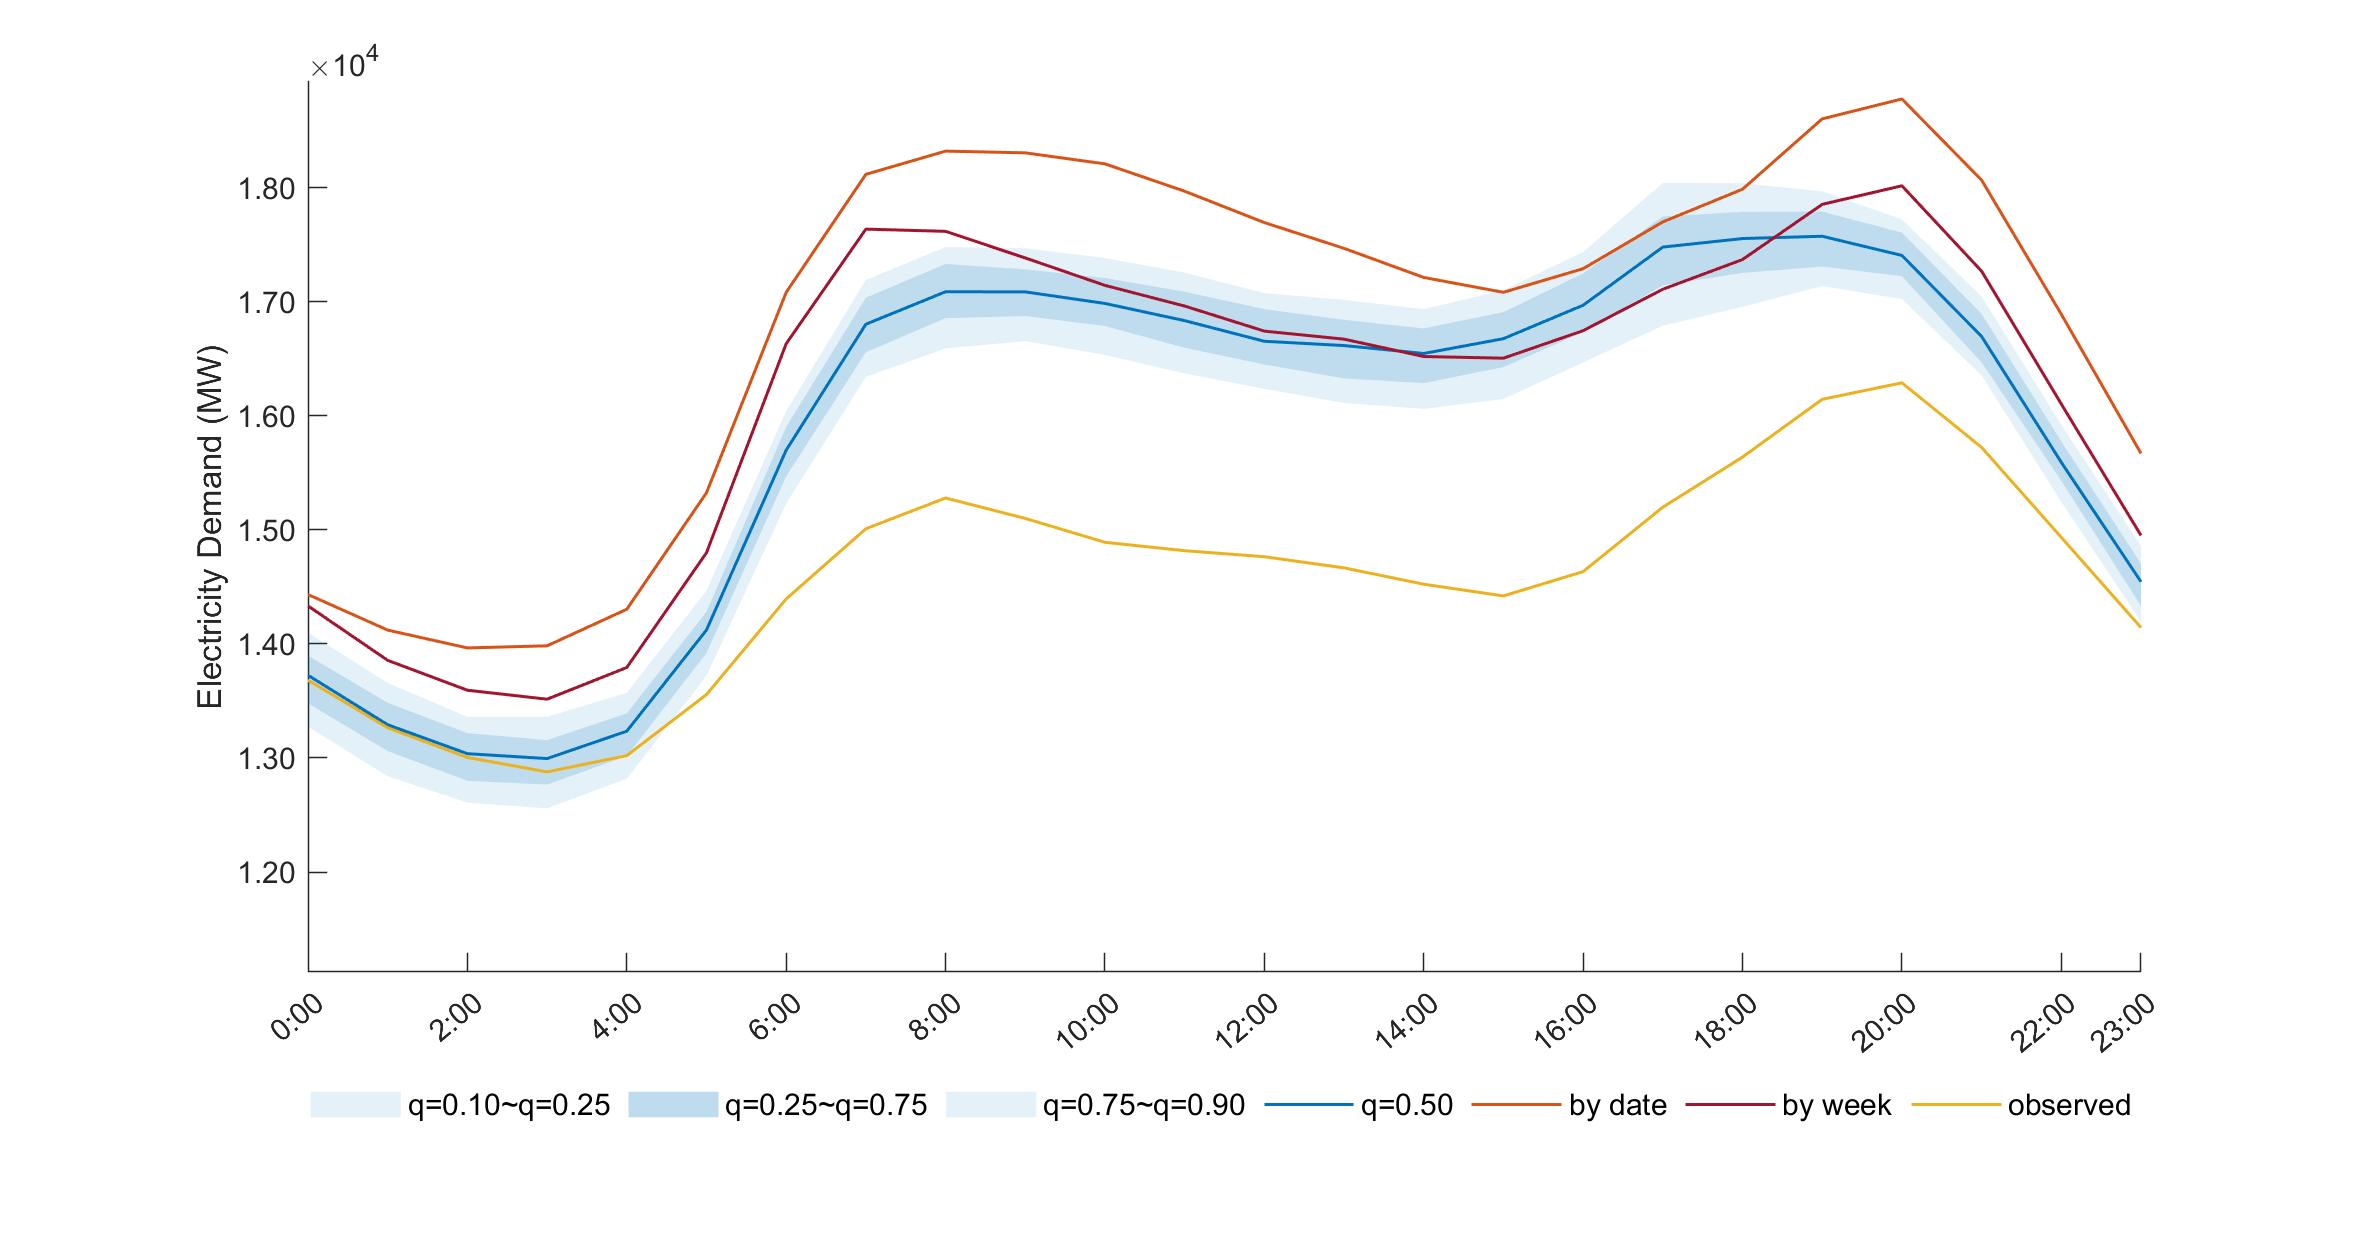
\includegraphics[width=0.8\textwidth]{figures/example_backcast.jpg}
  \caption{Example: Baseline and Observed Demand of NYISO} \label{fig:backcast_eg}
\end{figure}



\subsubsection{Regression Analysis}\label{subsec:eg_regression}

\covemda{} is also capable of regression analysis. The corresponding function \verb!OLS! and \verb!VAR! provide regression models in which users may acquire correlation figures between variables. See Section~\ref{sec:regression} for more information.

For example, to apply a linear OLS model to the social distancing data of CAISO, the user may enter:

\begin{Command}
>> t=basic_read('caiso_rto_lmp')

t =

  1462x25 table

       date       00:00     01:00     02:00             ...
    __________    ______    ______    ______            ...

    2017-01-19     21.53     21.69     20.86            ...
    2017-01-20     26.46     24.67     23.68            ...
    2017-01-21     30.83     28.37     28.19            ...
    2017-01-22     27.33     26.5      25.14            ...
                ...                  ...                ...

>> t=exchange_columns(t,1,4)

t =

  1462x25 table

    02:00     00:00     01:00        date    
    ______    ______    ______    __________            ...

    20.86     21.53     21.69     2017-01-19            ...
    23.68     26.46     24.67     2017-01-20            ...
    28.19     30.83     28.37     2017-01-21            ...
    25.14     27.33     26.5      2017-01-22            ...
            ...                  ...                    ...
            
>> b=OLS(t,3,'linear')
               OLS Regerssion Results 
====================================================
           Model:                      OLS
           Method:           Least Squares
           Date:      29-Jun-2021 17:17:08
           Time:                   0.007 s
           R-squared:                0.984
           Adj. R-squared:           0.984
           F-statistic:              46073.89
           Prob (F-statistic):     
====================================================
        coef        std err        t         P>|t|      
     -0.35065     0.099122      -3.5376   0.00041647
     -0.15432     0.018966      -8.1368    8.605e-16
       1.1334     0.019961       56.781            0


b =

     -0.35065
     -0.15432
       1.1334
\end{Command}

Users may check the feasibility of the regression by figures in the printed chart. One direct way is to check the \verb!t value! of the regress coefficients. As for the linear OLS above, the first coefficient has the \verb!t value! of -3.5376, meaning that the possibility of P greater than $|t|$ is $2.37 \times 10^-5 << 0.05$. This suggests that the regression is feasible, and if the value is greater than $0.05$, user may rethink about the feasibility of this regression.


%----------------------------------------
\clearpage
\section{Data Hub} \label{sec:datahub}
\covemda{} toolbox is designed to utilize the data sourced from COVID-EMDA+ (Coronavirus Disease - Electricity Market Data Aggregation+). COVID-EMDA+ is specifically designed to track the potential impacts of COVID-19 on the existing U.S. electricity markets. Many different data sources are merged and harmonized here in order to enable further interdisciplinary researches. 

\textbf{Note}: Historical data dating back to 2017 are included as time-series benchmarks.

\subsection{Data Category}
Five major components are included in the data hub: 
\begin{itemize}
	\item U.S. electricity market data. This part includes the generation mix, metered load profiles, day-ahead locational marginal prices data, as well as day-ahead load forecasting, congestion price, forced outage and renewable curtailment data.
    	\begin{quotation}
    	    Source: \href{http://oasis.caiso.com/mrioasis/logon.do}{CAISO}, \href{https://www.misoenergy.org/markets-and-operations/real-time--market-data/market-reports/}{MISO}, \href{https://www.iso-ne.com/markets-operations/iso-express}{ISO-NE}, \href{https://www.nyiso.com/energy-market-operational-data}{NYISO}, \href{https://dataminer2.pjm.com/list}{PJM}, \href{https://marketplace.spp.org/groups/operational_data}{SPP}, \href{http://www.ercot.com/}{ERCOT}, \href{https://www.eia.gov/beta/electricity/gridmonitor/dashboard/electric_overview/US48/US48}{EIA}, \href{http://www.energyonline.com/}{EnergyOnline}.
    	\end{quotation}
	\item Public health data. This part includes the COVID-19 confirmed cases, deaths data, infection rate and fatal rate.
    	\begin{quotation}
            Source: \href{https://github.com/CSSEGISandData/COVID-19}{John Hopkins CSSE}.
    	\end{quotation}
	\item Weather data. This part includes temperature, relative humidity, wind speed and dew point data. Typical weather stations are selected according to their geological locations and data quality.
        \begin{quotation}
            Source: \href{https://mesonet.agron.iastate.edu/request/download.phtml}{Iowa State Univ IEM}, \href{https://www.nws.noaa.gov/ost/asostech.html}{NOAA}.
        \end{quotation}
	\item Mobile device location data. This part includes social-distancing data and patterns of visits to Point of Interests (POIs). These data are derived by aggregating and processing the real-time GPS location of cellphone users by Census Block Group.
	    \begin{quotation}
	        Source: \href{https://docs.safegraph.com/docs}{Mobility Data From SafeGraph}.
	    \end{quotation}
	\item Satellite images. Night Time Light (NTL)	Satellite data, to be specific. This part includes the raw satellite image taken at night time in each area.
	    \begin{quotation}
	        Source: \href{https://ladsweb.modaps.eosdis.nasa.gov/missions-and-measurements/products/VNP46A1/}{NTL Images from NASA}.
	    \end{quotation}
\end{itemize}
NOTE: For some categories, multiple data sources are carefully gathered to ensure accuracy.
\subsection{Data Structure}
This data hub mainly contains five components: source data, released data, supplementary resources, parser codes, and quick start tutorials. We navigate this data hub as follows.

\begin{enumerate}
    \item All the data source files are archived in folder \verb!data_source!, while the cleaned, processed data are stored in folder \verb!data_release!.
    
    Daily updates containing the latest data would be properly classified by location. The file name convention of COVID-EMDA+ is: \verb!MARKET_AREA_CATEGORY.csv!, e.g. \verb!nyiso_nyc_load.csv! is a dataset of load profile in New York City from 2017 to present.
    \item Supplementary resources of several publication works and relevant projects including a series of extended data sources and analysis codes could be found in folder \verb!supplementary!.
    \item Basic parser codes (written in Python) to handle the source data are implemented in folder \verb!parser!.
    \item Some quick start for the dataset is also accessible in folder \verb!startup! and \verb!supplementary!.
\end{enumerate}




\subsection{Field Description}
As mentioned, \verb!data_release! folder contains all the cleaned and processed data. The file name follows the convention of \verb!MARKET\_AREA\_CATEGORY.csv!. 
All the files are organized in a wide csv table. Here are some tips to further demonstrate the data.
\subsubsection{Electricity Market Data}
\begin{itemize}
	\item Field \textit{date}: list all the date from 2017 to present. Format: \textit{YYYYmmdd}
	\item Field \textit{fuel}: only in generation mix dataset, represent the different fuel source used by generators. Possible values: \textit{coal, gas, oil, nuclear, hydro, wind, solar, export, other.} Different definitions in different electricity markets are harmonized.
	\item Field \textit{kind}: only in weather dataset, represent the type of measurement that is recorded in each corresponding row. Possible value: \textit{dwpc (dew point temperature), relh (relative humidity), sped (wind speed), tmpc (temperature)}.
	\item Field \textit{HH:MM}: represent the hourly time slot. For example, column ``08:00'' records the data of period 8AM to 9AM.
\end{itemize}
\subsubsection{COVID-19 Data}
\begin{itemize}
	\item Field \textit{date}: list all the date from Jan. 23, 2020 to present. Format: \textit{YYYYmmdd}
	\item Field \textit{accum\_confirm}: accmulated confirmed case number recorded for each date.
	\item Field \textit{new\_confirm}: newly confirmed case number for each date.
	\item Field \textit{infect\_rate}: infection ratio calculated for each date.
	\item Field \textit{accum\_death}: accmulated confirmed death number recorded for each date.
	\item Field \textit{new\_death}: newly confirmed death number for each date.
	\item Field \textit{fatal\_rate}: fatal rate calculated for each date.
\end{itemize}
\subsubsection{Visit Patterns to Point of Interests}
\begin{itemize}
	\item Field \textit{date}: list all the date from Dec.30, 2019 to present. Format: \textit{YYYYmmdd}
	\item Field \textit{Restaurant\_Recreaction}: daily total number of visits to Restaurant and Recreaction places. 
	\item Field \textit{Grocery\_Pharmacy}: daily total number of visits to Grocery and Pharmacy places.
	\item Field \textit{Retail}: daily total number of visits to Retail places. 
\end{itemize}
\subsubsection{Social Distancing}
\begin{itemize}
	\item Field \textit{date}: list all the date from Jan. 1, 2020 to present. Format: \textit{YYYYmmdd}
	\item Field \textit{completely\_home\_device\_count\_percentage}: percentage of devices that stay at home 24 hours out of all devices.
	\item Field \textit{median\_home\_dwell\_time\_percentage}: median proportion of home dwell time in one day.
	\item Field \textit{part\_time\_work\_behavior\_devices\_percentage}: percentage of devices that go to workplaces for 3 to 6 hours out of all devices.
	\item Field \textit{full\_time\_work\_behavior\_devices\_percentage}: percentage of devices that go to workplaces for more than 6 hours out of all devices.
	\item Field \textit{completely\_home\_device\_count}: count of devices that stay at home 24 hours.
	\item Field \textit{device\_count}: total count of devices.
	\item Field \textit{part\_time\_work\_behavior\_devices\_count}: count of devices that go to workplaces for 3 to 6 hours.
	\item Field \textit{full\_time\_work\_behavior\_devices\_count}: count of devices that go to workplaces for more than 6 hours.
\end{itemize}
\subsection{Quality Control}
\begin{figure}[htbp]
	\centering
	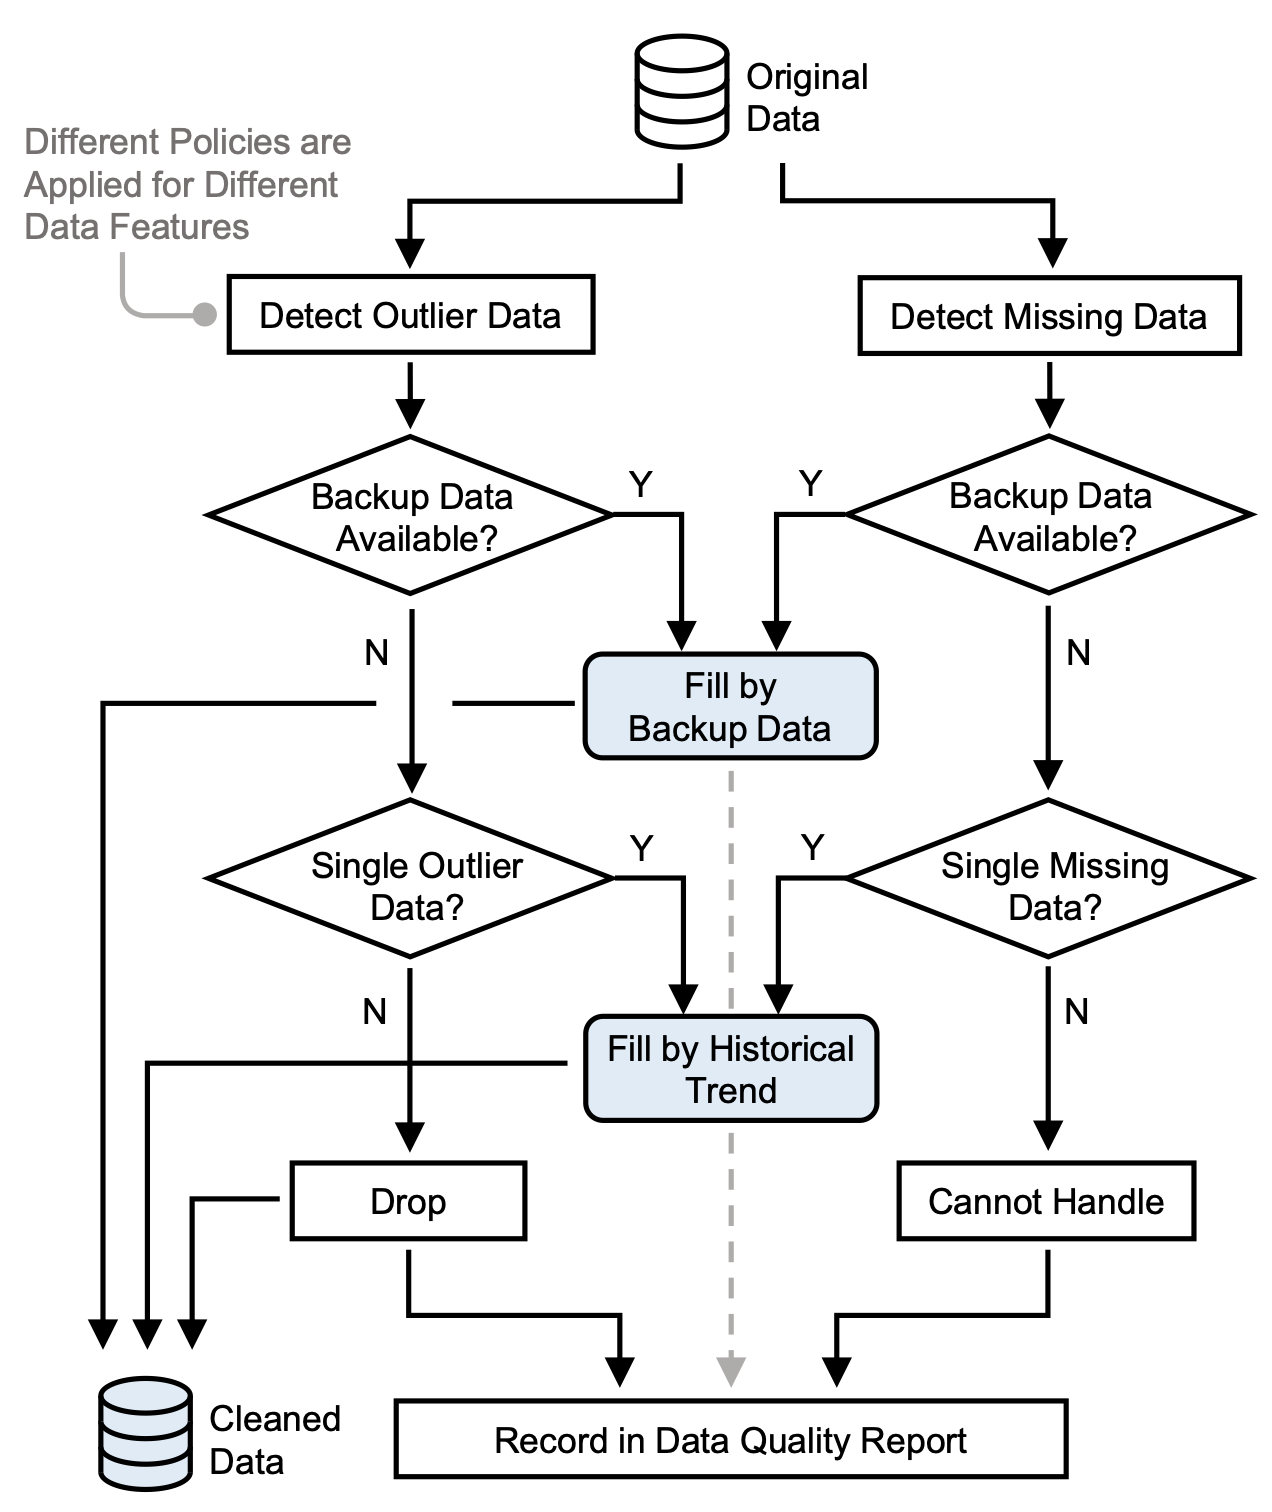
\includegraphics[width=.5\textwidth]{figures/data-quality-control.png}
	\caption{Details of Data Quality Control.}

	\label{fig:dataqualitycontrol}
\end{figure}	

To provide reliable and easy-to-use dataset, a series of data checking and cleaning procedures are implemented.
Data quality control mainly includes two aspects: outlier detection and missing data recovery. Backup data and historical trend are used to achieve both functions, as shown in Figure~\ref{fig:dataqualitycontrol}.
\begin{itemize}
	\item Single missing data (most frequent) are filled by linear interpolation. For consecutive missing data (for example, consecutive missing dates, which are very rare), data from the EIA or EnergyOnline are carefully supplemented.
	\item Outlier data samples are automatically detected when they are beyond 5 times or below 20\% of the associated daily average value. Exceptions such as price spikes and negative prices in LMP data are carefully handled.
	\item Duplicate data are dropped, only the first occurrence of each data sample is kept.
\end{itemize}

\textbf{NOTE}: For those that cannot be handled, we record them in the data quality report as shown in the GitHub as well. It is recommended to check the \href{https://github.com/tamu-engineering-research/COVID-EMDA/tree/master/data_release}{report} to get some knowledge of data released before you use the datasets. The Table~\ref{tab:dataqualityreport} shows a snapshot of the report by Jun.6, 2021.

\begin{table}[htbp]
	\scriptsize
	\centering
	\caption{Data Quality Report(Snapshot by Jun.6, 2021).}
	\label{tab:dataqualityreport}
	\begin{tabular}{llllp{0.3\textwidth}}
	\toprule
	\multicolumn{1}{l}{Dataset Name} & \multicolumn{1}{l}{Market} & \multicolumn{1}{l}{Area} & \multicolumn{1}{l}{Category} & \multicolumn{1}{l}{Missing Dates}                                                           \\
	\midrule
	caiso\_rto\_genmix.csv                    & CAISO                               & RTO Level                         & Generation Mix                        & Sep 23 - Oct 3, 2019                                                                                                         \\
	caiso\_rto\_lmp.csv                       & CAISO                               & RTO Level                         & Day-Ahead LMP                         & Jan 1 - Jan 18, 2017; Oct 5, Oct 9, 2020                                                                                     \\
	caiso\_la\_load.csv                       & Near CAISO                          & Los Angeles                       & Hourly Load                           & Nov 5, 2017; Jan 11 - 12, Jun 29 - 30, Jul 1 - 9, Sep 27, Nov 4, 2018; Mar 10, Nov 3, 2019; Mar 8, Nov 1, 2020; Mar 14, 2021 \\
	caiso\_la\_weather                        & CAISO                               & Los Angeles                       & Weather                               & Apr 7 - 8, 2021                                                                                                              \\
	ercot\_rto\_load.csv                      & \textbf{ERCOT}                      & \textbf{RTO Level}                & \textbf{Hourly Load}                  & Dec 13, 2020                                                                                                                 \\
	ercot\_houston\_load.csv                  & ERCOT                               & Houston City                      & Hourly Load                           & Dec 13, 2020                                                                                                                 \\
	ercot\_houston\_weather.csv               & ERCOT                               & Houston City                      & Weather                               & Feb 15 - 16, 2020                                                                                                            \\
	isone\_rto\_genmix.csv                    & ISO-NE                              & RTO Level                         & Generation Mix                        & Apr 30, 2018; Jun 21, Oct 30-31, Dec 06, 2020                                                                                \\
	isone\_rto\_load.csv                      & ISO-NE                              & RTO Level                         & Hourly Load                           & Dec 17, 2020                                                                                                                 \\
	pjm\_rto\_genmix.csv                      & PJM                                 & RTO Level                         & Generation Mix                        & Mar 29 - Apr 2, 2017                                                                                                         \\
	spp\_rto\_genmix.csv                      & SPP                                 & RTO Level                         & Generation Mix                        & Mar 29, 2019                                                                                                                 \\
	spp\_kck\_weather.csv                     & SPP                                 & Kansas City                       & Weather                               & Sep 22 - 23                \\                                                                                                 
	\bottomrule
	\end{tabular}
	\end{table}










%--------------------------------
\newpage
\section{Baseline Estimation} \label{sec:baseline}

Baseline refers to the basis of comparison with or without certain factor\cite{wijaya2014bias}\cite{mohajeryami2016error}. Here, baseline estimation provides the control group for analysis of the impact of COVID-19 on electricity consumption. Traditional method for baseline estimation usually involves selecting specific days of the same patterns in the past, and integrating corresponding historical data. Such methods rely heavily on the principle for similar date selection, reducing their robustness and accuracy. By contrast, \textbf{ensemble backcast model} utilizes deep neural networks and multi-dimensional historical data to produce a more reliable baseline. In practice, as the default algorithm for baseline estimation in \covemda{}, it accurately reflects the normal trend of electricity consumption in the absence of the pandemic.

\covemda{} function \verb!cal_baseline! provides a uniform tool for baseline calculation by either date alignment, week index alignment or backcast estimation. In addition, \covemda{} offers a tool for simple visualization of different baseline estimation methods: \verb!plot_baseline!. This function calculates the load baseline with different estimation methods by \verb!cal_baseline!, and plots them in one graph. Unlike \verb!cal_baseline!, here multiple methods can be appointed for comparison. See Section~\ref{func:cal_baseline} and Section~\ref{func:plot_baseline} for more detail.



\subsection{Date and Week Alignment}

Date alignment for baseline estimation refers to calculating the load baseline by searching for the load data of the exact same date and month in the previous year. This calculation process is performed by \covemda{} function \verb!cal_baseline_by_dates!. See Section~\ref{func:cal_baseline_by_dates} for more detail.

Week index alignment for baseline estimation refers to calculating the load baseline by searching for the load data of the exact same week and day of week in the previous year. This calculation process is performed by \covemda{} function \verb!cal_baseline_by_week_index!. See Section~\ref{func:cal_baseline_by_week_index} for more detail.



\subsection{Ensemble Backcast Estimation}
The \textbf{Ensemble Backcast Model} is used to estimate the electricity consumption profile in the absence of COVID-19 pandemic, so that the comparison between the model and actual metered electricity consumption can be used to quantify the impact of COVID-19.

A backcast model is expressed as a function that maps potential factors that may affect electricity consumption level, including weather variables (such as temperature, humidity and wind speed), date of year, and economic prosperity (yearly GDP growth rate) to the estimated electricity consumption. Given a group of backcast models, ensemble forecasting is widely recognized as the best approach to provide rich interval information\cite{gosink2013characterizing}. A group of backcast models for the daily average electricity consumption can be described by

\begin{equation*}
  \hat L_{md}=\frac{1}{N}\sum\limits_{i=1}^N \hat f_i(C_{md}, T_{mdq}, H_{mdq}, S_{mdq}, E),\forall m,d
\end{equation*}

where 
\begin{itemize}
  \item $C_{md}$ is the calendar information including month, day, weekday, and holiday flag.
  \item $\hat L_{md}$ is the estimated daily average electricity consumption for month $m$ and day $d$.
  \item $\hat f_i$ is the $i$-th backcast model.
  \item $T_{mdq},H_{mdq},S_{mdq}$ are temperature, humidity and wind speed within the selected quantiles $q$.
  \item $E$ is the estimated GDP growth rate.
\end{itemize}
We typically include 25\%, 50\% (average value), 75\% and 100\%(maximium) quantiles, and the final inputs should be decided based on the the data after extensive testing.

In \covemda{}, this calculation process is performed by function \verb!cal_baseline_by_backcast!. See Section~\ref{func:cal_baseline_by_backcast} for more detail.



\subsection{Abnormal Price Index}\label{subsec:abnormal_price_index}

Locational marginal prices play a crucial role in electricity markets and contribute to balancing generation and demand efficiently. Since these prices are relatively stochastic in nature, it is unsatisfactory to analyze them in the same way as electricity demand\footnote{the uncertainty intervals will be very wide}. Thus, the abnormal price index is developed to provide a more reliable tool for price analysis, which is defined as follows,
\begin{equation*}
  I(\lambda_{ymdt})=|2\hat F_m(\lambda_{ymdt})-1|, \forall y,m,d,t,
\end{equation*}
where $\lambda_{ymdt}$ is the day-ahead locational marginal price of year $y$, month $m$, day $d$, and hour $t$. $I(\cdot)$ is the proposed index, which lies between zero and one. This index quantifies the abnormality of a typical price, and a larger index value represents a more unusual observation. $\hat F_m(\cdot)$ is the cumulative distribution function for the prices in month $m$.\footnote{Which are more stable for analyzing these price changes. See the reason in \cite{quantitaveassess}}.

The statistical meaning of the above index is explained by the probability density function shown in Figure~\ref{fig:abnormal_price_index}. For a given price, the index donates a possibility that measures how close this price is to the mean value. For example, if a price observation is located within the 25\% and 75\% quantiles, we obtain an index value below 0.5, which is considered normal.
\begin{figure}
  \centering
  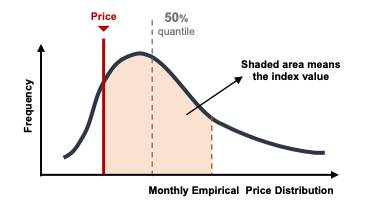
\includegraphics[width=.8\textwidth]{figures/abnormal_price_index.png}
  \caption{Statistical illustration of the proposed abnormal price index. The basic idea is to show how near a price observation is to the mean value. This index can eliminate some stochastic factors when assessing price changes. The index value lies in [0,1], and a larger value means a higher possibility of abnormality.}
  \label{fig:abnormal_price_index}
\end{figure}

In \covemda{}, the abnormal price index is calculated by function \verb!cal_abnormal_price_index!. More detail is available in Section~\ref{func:cal_abnormal_price_index}.

\subsection{Price Distribution Change Across Different Areas}\label{subsec:cal_distribution_diff}

To conduct a cross-market comparison, a Wasserstein probability distance \cite{carrillo2004wasserstein}\cite{kantorovich2006translocation} metric to quantify the price change during the pandemic. The price change for year $y$ can be formulated as follows.
\begin{equation*}
    s_y=\text{WD}(\text{Vec}(\lambda_{ymdt})-\text{Vec}(\lambda_{hist})),\quad\forall y    
\end{equation*}
where $s_y$ donates the price change for year $y$ that is calculated by a Wasserstein distance function WD($\cdot$). Vec($\cdot$) is a vectorization function to place all the price data from March to mid-July in a one-dimensional array. $\lambda_{hist}$ represents all the historical price data accordingly.

In \covemda{}, the price distribution distance is calculated by function \verb!cal_distribution_diff!. More detail is available in \ref{func:cal_distribution_diff}.

\subsection{Excess Change Rate of Renewable}\label{subsec:excess_change_rate}

One simple way to quantify the changes of renewable share during the COVID-19 pandemic is to make a linear assumption of its growth rate. Based on the assumption, the \textbf{excess change rate} is defined as the relative change rate between the observed renewable share and this estimation:

\begin{equation*}
    \eta=\left(\frac{r_{2020}}{2r_{2019}-r_{2018}}-1\right)\times100\%
\end{equation*}
where $\eta$ is the excess change rate, and $r_{2018}\sim r_{2020}$ are the market shares of renewable energy observed in 2018, 2019 and 2020.

In \covemda{}, the excess change rate of renewable in various markets is provided by function \verb!cal_excess_change_rate!. This function reads the generation mix data from the data hub, and calculates the corresponding excess change rate according to the formula above. More detail is available in Section~\ref{func:cal_excess_change_rate}.



\subsection{Functions}

\subsubsection{\texttt{cal\_baseline}}\label{func:cal_baseline}

\begin{Code}
function t_output=cal_baseline(market,varargin)
\end{Code}

\covemda{} function \verb!cal_baseline! provides a uniform tool for baseline calculation by either date alignment, week index alignment or backcast estimation. By default, this function returns the load baseline (as a table or several tables if multiple quantiles are calculated) of specified ISO or city (if \verb!City! is specified) by backcast estimation from 2020-02-01 to 2020-06-30. The user needs to specify the value of name-value pair argument \verb!Method! to alter calculation method (\verb!'date', 'week', 'backcast'!), or \verb!DateRangeCovid! to change the output date range.

In practice, since this function calls the following low-level functions concerning baseline estimation, all the other arguments are passed on to them. For instance, to train the ensemble backcast model with specified model numbers before estimating baseline, the user may call the function like this:

\begin{Command}
>> cal_baseline('nyiso','TrainModel',1,'ModelNum',[10,3]);
\end{Command}

Although argument \verb!TrainModel! and \verb!ModelNum! belong to the low-level function \verb!cal_baseline_by_backcast!, it is recommended to specify them when calling high-level function \verb!cal_baseline!. See Table~\ref{tab:cal_baseline} for a full list of arguments.

\begin{table}[!ht]
  \centering
  \begin{threeparttable}
    \caption{Cal Baseline Options}
    \label{tab:cal_baseline}
    \footnotesize
    \begin{tabular}{lp{.3\textwidth}p{0.5\textwidth}}
      \toprule
      Name & Type & Description \\
      \midrule
      Method & \begin{tabular}[t]{l}
        character array \\
        string    \\
      \end{tabular} & Method for baseline estimation, specified as \verb!'date'!, \verb!'week'! or \verb!'backcast'!.   \\
       & & \begin{tabular}[t]{l @{ -- } l}
        Default & \verb!'backcast'!. \\
      \end{tabular}                         \\
      \midrule
      DateRangeCovid & \begin{tabular}[t]{l}
        datetime array \\
        string array    \\
        cell array of character vectors \\
      \end{tabular} & Range of time for baseline estimation.  \\
       & & \begin{tabular}[t]{l @{ -- } l}
        Default & \verb!{'2020-02-01','2020-06-30'}!. \\
        Example & \verb!{'2020-04-01','2020-04-30'}!  \\
                & \verb!'2020-04-01'!  \\
      \end{tabular} \\
      \midrule
      Others & & See Section~\ref{func:cal_baseline_by_dates}, Section~\ref{func:cal_baseline_by_week_index} and Section~\ref{func:cal_baseline_by_backcast}. \\
      \bottomrule
    \end{tabular}
  \end{threeparttable}
\end{table}



\subsubsection{\texttt{plot\_baseline}}\label{func:plot_baseline}

\begin{Code}
function gr_handles=plot_baseline(market,varargin)
\end{Code}

\covemda{} offers a tool for simple visualization of different baseline estimation methods: \verb!plot_baseline!. This function calculates the load baseline with different estimation methods by \verb!cal_baseline!, plots them in one graph, and returns the handles of graphic objects. The user can appoint the methods to be plotted by specifying the value of name-value pair argument \verb!Method!. Unlike \verb!cal_baseline!, here the parameter value can be multiple method names in the form of cell arrays or string arrays, etc. If so, \verb!cal_baseline! is called for each estimation method.

The user can specify the bin and method for resampling data of the plot by argument \verb!ResampleBin!, \verb!ResampleMethod! as well, just like the visualization functions in Section~\ref{sec:visual}. See Table~\ref{tab:plot_baseline} for a full list of arguments.

\begin{table}[!ht]
  \centering
  \begin{threeparttable}
    \caption{Plot Baseline Options}
    \label{tab:plot_baseline}
    \footnotesize
    \begin{tabular}{lp{.3\textwidth}p{0.5\textwidth}}
      \toprule
      Name & Type & Description \\
      \midrule
      Method & \begin{tabular}[t]{l}
        cell array of character vectors \\
        string array \\
      \end{tabular} & Methods for baseline estimation, specified as \verb!'date'!, \verb!'week'! and(or) \verb!'backcast'!.   \\
       & & \begin{tabular}[t]{l @{ -- } l}
        Default & \verb!["backcast", "date", "week"]!. \\
        Example & \verb!'backcast'! \\
      \end{tabular}                         \\
      \midrule
      ResampleBin & \begin{tabular}[t]{l}
        string            \\
        character vectors \\
      \end{tabular} & Binning scheme for resampling. \\
       & & \begin{tabular}[t]{l @{ -- } l}
        Default & \verb!'none'!. \\
      \end{tabular}                         \\
      \midrule
      ResampleMethod & \begin{tabular}[t]{l}
        string            \\
        character vectors \\
      \end{tabular} & Computation method for resampling. \\
      & & \begin{tabular}[t]{l @{ -- } l}
        Default & \verb!'mean'!. \\
      \end{tabular}                         \\
      \midrule
      Others & & See Section~\ref{func:cal_baseline}. \\
      \bottomrule
    \end{tabular}
  \end{threeparttable}
\end{table}



\subsubsection{\texttt{cal\_baseline\_by\_dates}}\label{func:cal_baseline_by_dates}

\begin{Code}
function t_output=cal_baseline_by_dates(market,dr_Covid,varargin)
\end{Code}

If \verb!Method! is specified as \verb!date!, function \verb!cal_baseline! calculates the load baseline by searching for the load data of the exact same date and month in the previous year, for every day in \verb!DateRangeCovid!. This calculation process is performed by function \verb!cal_baseline_by_dates!. It returns a table containing the dates and load baseline data.

The only additional argument here is \verb!City!, specified as one of the seven abbreviations: \verb!'la'!,  \verb!'houston'!, \verb!'boston'!, \verb!'nyc'!, \verb!'chicago'!, \verb!'phila'! and \verb!'kck'!, or \verb!'rto'! (default) if the user needs the result for the entire market.



\subsubsection{\texttt{cal\_baseline\_by\_week\_index}}\label{func:cal_baseline_by_week_index}

\begin{Code}
function t_output=cal_baseline_by_week_index(market,dr_Covid,varargin)
\end{Code}

If \verb!Method! is specified as \verb!week!, function \verb!cal_baseline! calculates the load baseline by searching for the load data of the exact same week and day of week in the previous year, for every day in \verb!DateRangeCovid!. This calculation process is performed by function \verb!cal_baseline_by_week_index!. It returns a table containing the dates and load baseline data.

The only additional argument here is \verb!City! as well, specified as one of the seven abbreviations: \verb!'la'!,  \verb!'houston'!, \verb!'boston'!, \verb!'nyc'!, \verb!'chicago'!, \verb!'phila'! and \verb!'kck'!, or \verb!'rto'! (default) if the user needs the result for the entire market.



\subsubsection{\texttt{cal\_baseline\_by\_backcast}}\label{func:cal_baseline_by_backcast}

\begin{Code}
function t_YPreds=cal_baseline_by_backcast(market,dr_Covid,varargin)
\end{Code}

If \verb!Method! is specified as \verb!backcast!, function \verb!cal_baseline! calculates the load baseline by either training new models or using existing models. This calculation process is performed by function \verb!cal_baseline_by_backcast!. If only one single quantile is appointed, this function returns a table containing the dates and load baseline data like the others. However, if multiple quantiles are appointed, this function returns a table whose first column is the quantiles, and each element in the second column is a table containing dates and baseline for corresponding quantile. All parameter names are listed in Table~\ref{tab:cal_baseline_by_backcast}.

In general, this function consists of 3 or 6 steps (depends on whether to train models or not). If the user chooses to train a new model, the function

\begin{enumerate}
    \item imports training data and splits training and testing set (\verb!backcast_import_data!);
    \item trains two-layer deep neural network models using training set with validation (\verb!backcast_scan_training!);
    \item tests all the models and selects the best ones using testing set (\verb!backcast_test_model!);
    \item saves trained models and summary (\verb!basic_backcast_save_file!);
    \item imports data for baseline estimation (\verb!backcast_import_data!);
    \item calculates the load baseline with quantiles (\verb!backcast_scan_prediction!).
\end{enumerate}

If the user chooses not to train models but to use pre-trained models, the function

\begin{enumerate}
    \item imports existing models (\verb!basic_backcast_import_models!);
    \item imports data for baseline estimation (\verb!backcast_import_data!);
    \item calculates the load baseline with quantiles (\verb!backcast_scan_prediction!).
\end{enumerate}

\begin{table}[!ht]
  \centering
  \begin{threeparttable}
    \caption{Cal Baseline By Backcast Options}
    \label{tab:cal_baseline_by_backcast}
    \footnotesize
    \begin{tabular}{lp{.3\textwidth}p{0.5\textwidth}}
      \toprule
      Name & Type & Description \\
      \midrule
      City & \begin{tabular}[t]{l}
        string    \\
        character array \\
      \end{tabular} & Abbreviation of the target city or \verb!'rto'! for the entire market.  \\
       & & \begin{tabular}[t]{l @{ -- } l}
        Default & \verb!'rto'!. \\
      \end{tabular}                         \\
      \midrule
      TrainModel & integer value & Train (1) or not train (0) models.   \\
       & & \begin{tabular}[t]{l @{ -- } l}
        Default & 0. \\
      \end{tabular}                         \\
      \midrule
      ImportNum & integer value or \verb!'latest'! & The id of the existing model to be imported. Only effective when TrainModel=0.  \\
       & & \begin{tabular}[t]{l @{ -- } l}
        Default & \verb!'latest'!. \\
      \end{tabular}                         \\
      \midrule
      DateRangeTrain & \begin{tabular}[t]{l}
        datetime array \\
        string array    \\
        cell array of character vectors \\
      \end{tabular} & Range of time for model training. Only effective when TrainModel=1.  \\
       & & \begin{tabular}[t]{l @{ -- } l}
        Default & \verb!{'2018-02-01','2020-01-31'}!. \\
        Example & \verb!{'2018-01-01','2019-12-31'}!  \\
                & \verb!["2018-01-01","2019-12-31"]!  \\
      \end{tabular} \\
      \midrule
      ModelNum & two-element numeric vector & The number of models to be tested and selected. Only effective when TrainModel=0.  \\
       & & \begin{tabular}[t]{l @{ -- } l}
        Default & \verb![800, 200]!. \\
      \end{tabular}                         \\
      \midrule
      SaveModel & integer value & Indicator to save trained models in \matlab{} .asv files. Save(1) or not save(0). Only effective when TrainModel=0.  \\
       & & \begin{tabular}[t]{l @{ -- } l}
        Default & 1. \\
      \end{tabular}                         \\
      \midrule
      SaveModelONNX & integer value & Indicator to save trained models in .onnx files. Save(1) or not save(0). Only effective when TrainModel=0.  \\
       & & \begin{tabular}[t]{l @{ -- } l}
        Default & 0. \\
      \end{tabular}                         \\
      \midrule
      SaveSummary & integer value & Indicator to save summary of trained models. Save(1) or not save(0). Only effective when TrainModel=0.  \\
       & & \begin{tabular}[t]{l @{ -- } l}
        Default & 1. \\
      \end{tabular}                         \\
      \midrule
      Others & & See Section~\ref{func:backcast_import_data}, Section~\ref{func:backcast_scan_training}, Section~\ref{func:backcast_test_model} and Section~\ref{func:backcast_scan_prediction}. \\
      \bottomrule
    \end{tabular}
  \end{threeparttable}
\end{table}



\subsubsection{\texttt{backcast\_import\_data}}\label{func:backcast_import_data}

\begin{Code}
function [t_XTrainandtest,t_YTrainandtest,t_XTrainandvalid,t_YTrainandvalid,
t_XTest,t_YTest]=backcast_import_data(market,dr_Trainandtest,varargin)
\end{Code}

Function \verb!backcast_import_data! is the subfunction of \verb!cal_baseline_by_backcast!, in charge of importing data for training, validation and testing of the ensemble backcast model. \verb!t_XTrainandtest! and \verb!t_YTrainandtest! are the training (including validation) and testing set, and the others are training-validation set and testing set separated from each other, i.e., the union of the last four equals the first two.

The only additional argument here is \verb!City!, specified as one of the seven abbreviations: \verb!'la'!,  \verb!'houston'!, \verb!'boston'!, \verb!'nyc'!, \verb!'chicago'!, \verb!'phila'! and \verb!'kck'!, or \verb!'rto'! (default) if the user needs the result for the entire market.



\subsubsection{\texttt{backcast\_scan\_training}}\label{func:backcast_scan_training}

\begin{Code}
function t_net=backcast_scan_training(t_XTrainandvalid,t_YTrainandvalid,
model_num,varargin)
\end{Code}

Function \verb!backcast_scan_training! is the subfunction of \verb!cal_baseline_by_backcast!, in charge of training the deep neural networks. This function trains \verb!model_num! deep neural networks with two hidden layers and random number of hidden units, determined by argument \verb!numHiddenUnits! and \verb!RandVariation!. The return value of this function is a table of all the trained models, along with their parameters, validation accuracy and corresponding scalers. All parameter names are listed in Table~\ref{tab:backcast_scan_training}.

\begin{table}[!ht]
  \centering
  \begin{threeparttable}
    \caption{Backcast Scan Training Options}
    \label{tab:backcast_scan_training}
    \footnotesize
    \begin{tabular}{lp{.3\textwidth}p{0.5\textwidth}}
      \toprule
      Name & Type & Description \\
      \midrule
      numHiddenUnits & two-element numeric vector & The number of hidden units in the two full connection layers. Only effective when TrainModel=0.  \\
       & & \begin{tabular}[t]{l @{ -- } l}
        Default & \verb![32, 64]!. \\
      \end{tabular}                         \\
      \midrule
      TrainVerbose & integer value & Indicator to display training progress information. No display(0), brief display(1) or detailed display(2). Only effective when TrainModel=0.  \\
       & & \begin{tabular}[t]{l @{ -- } l}
        Default & 1. \\
      \end{tabular}                         \\
      \midrule
      RandVariation & double value in (0,1) & Relative range (1-RandVariation, 1+RandVariation) of random variation of model parameters numHiddenUnits for scan training. Only effective when TrainModel=0.  \\
       & & \begin{tabular}[t]{l @{ -- } l}
        Default & 0.2. \\
      \end{tabular}                         \\
      \bottomrule
    \end{tabular}
  \end{threeparttable}
\end{table}



\subsubsection{\texttt{backcast\_test\_model}}\label{func:backcast_test_model}

\begin{Code}
function [t_net_all,t_net_sel]=backcast_test_model(t_net_all,t_XTest,
t_YTest,model_sel,varargin);
\end{Code}

Function \verb!backcast_test_model! is the subfunction of \verb!cal_baseline_by_backcast!, in charge of selecting the best deep neural networks. This function selects the best \verb!model_sel! models using the testing set. \verb!t_net_sel! is a table of the selected models, and \verb!t_net_all! is still the table of all models, with the information (testing accuracy, sign of selection) of the test.

The only additional argument here is \verb!TrainVerbose!, which is the same as the one in Section~\ref{func:backcast_scan_training}.



\subsubsection{\texttt{backcast\_scan\_prediction}}\label{func:backcast_scan_prediction}

\begin{Code}
function t_YPreds=backcast_scan_prediction(t_net,t_XPred,varargin)
\end{Code}

Function \verb!backcast_scan_prediction! is the subfunction of \verb!cal_baseline_by_backcast!, in charge of calculating baseline using the ensemble backcast model. It returns a table containing the dates and load baseline data. All parameter names are listed in Table~\ref{func:backcast_scan_prediction}.

\begin{table}[!ht]
  \centering
  \begin{threeparttable}
    \caption{Backcast Scan Prediction Options}
    \label{tab:backcast_scan_prediction}
    \footnotesize
    \begin{tabular}{lp{.3\textwidth}p{0.5\textwidth}}
      \toprule
      Name & Type & Description \\
      \midrule
      Quantile & numeric vector in (0,1) & Quantiles to be calculated in scan prediction. \\
       & & \begin{tabular}[t]{l @{ -- } l}
        Default & \verb![0.1, 0.25, 0.5, 0.75, 0.9]!. \\
        Example & 0.5   \\
      \end{tabular}                         \\
      \midrule
      PredictVerbose & integer value & Indicator to display prediction progress information. No display(0) or brief display(1).  \\
       & & \begin{tabular}[t]{l @{ -- } l}
        Default & 1. \\
      \end{tabular}                         \\
      \bottomrule
    \end{tabular}
  \end{threeparttable}
\end{table}



\subsubsection{\texttt{cal\_abnormal\_price\_index}}\label{func:cal_abnormal_price_index}

\begin{Code}
function output=cal_abnormal_price_index(market,varargin)
\end{Code}

Function \verb!cal_abnormal_price_index! calculates the proposed abnormal index in Section~\ref{subsec:abnormal_price_index}. The output is a table containing abnormal price index and corresponding date. All parameter names are listed in Table~\ref{tab:cal_abnormal_price_index}.

\begin{table}[!ht]
  \centering
  \begin{threeparttable}
    \caption{Cal Abnormal Price Index and Cal Distribution Diff Options}
    \label{tab:cal_abnormal_price_index}
    \footnotesize
    \begin{tabular}{lp{.3\textwidth}p{0.5\textwidth}}
      \toprule
      Name & Type & Description \\
      \midrule
      DateRange & \begin{tabular}[t]{l}
        datetime array \\
        string array    \\
        cell array of character vectors \\
      \end{tabular} & Range of time for index calculation. \\
       & & \begin{tabular}[t]{l @{ -- } l}
        Default & \verb!{'2020-03-01','2020-07-15'}!. \\
        Example & \verb!{'2020-01-01','2020-12-31'}!  \\
                & \verb!["2020-01-01","2020-12-31"]!  \\
      \end{tabular} \\
      \midrule
      City & \begin{tabular}[t]{l}
        string    \\
        character array \\
      \end{tabular} & Abbreviation of the target city or \verb!'rto'! for the entire market.  \\
       & & \begin{tabular}[t]{l @{ -- } l}
        Default & \verb!'rto'!. \\
      \end{tabular}                         \\
      \bottomrule
    \end{tabular}
  \end{threeparttable}
\end{table}



\subsubsection{\texttt{cal\_distribution\_diff}}\label{func:cal_distribution_diff}

\begin{Code}
function output=cal_distribution_diff(market,varargin)
\end{Code}

Function \verb!cal_distribution_diff! provides an indicator for the difference of price distribution with data from the previous year as baseline. It adopts Wasserstein distance as the measurement method. All parameter names are listed in Table~\ref{tab:cal_abnormal_price_index}.



\subsubsection{\texttt{cal\_excess\_change\_rate}}\label{func:cal_excess_change_rate}

\begin{Code}
function output=cal_excess_change_rate(market,varargin)
\end{Code}

Function \verb!cal_excess_change_rate! calculates the proposed abnormal index in Section~\ref{subsec:excess_change_rate}. The return value is the proposed excess change rate of renewable of the specified market. All parameter names are listed in Table~\ref{tab:cal_excess_change_rate}.

\begin{table}[!ht]
  \centering
  \begin{threeparttable}
    \caption{Cal Excess Change Rate Options}
    \label{tab:cal_excess_change_rate}
    \footnotesize
    \begin{tabular}{lp{.3\textwidth}p{0.5\textwidth}}
      \toprule
      Name & Type & Description \\
      \midrule
      DateRange & \begin{tabular}[t]{l}
        datetime array \\
        string array    \\
        cell array of character vectors \\
      \end{tabular} & Range of time for index calculation. \\
       & & \begin{tabular}[t]{l @{ -- } l}
        Default & \verb!{'2017-01-01','2020-07-15'}!. \\
        Example & \verb!{'2017-01-01','2020-12-31'}!  \\
                & \verb!["2017-01-01","2020-12-31"]!  \\
      \end{tabular} \\
      \midrule
      City & \begin{tabular}[t]{l}
        string    \\
        character array \\
      \end{tabular} & Abbreviation of the target city or \verb!'rto'! for the entire market.  \\
       & & \begin{tabular}[t]{l @{ -- } l}
        Default & \verb!'rto'!. \\
      \end{tabular}                         \\
      \bottomrule
    \end{tabular}
  \end{threeparttable}
\end{table}



\subsection{Examples}

In this section, we introduce the usage of the functions above with several examples. It is recommended to use feature-oriented high-level functions (see \ref{subsec:func_list}), and the following explanations and instructions are designed for them.

All high-level functions mentioned above (\verb!cal_baseline!, \verb!plot_baseline!, \verb!cal_abnormal_price_index!, \verb!cal_distribution_diff! and \verb!cal_excess_change_rate!) have similar input forms and can be used similarly. To be specific, the first input argument (market name) is compulsory, and all the other input arguments are optional. The market name is specified as one of the seven terms:

\begin{center}
  \verb!'caiso' | 'ercot' | 'isone' | 'miso' | 'nyiso' | 'pjm' | 'spp'!
\end{center}

As long as the market name is given, a basic version of the desired result can be simply obtained, which is illustrated in Section~\ref{subsec:eg_baseline}. All the other input arguments should be in the form of \textbf{name-value pairs} for the function to correctly recognize.

\begin{Command}
cal_baseline(market,'argument_name1',argument_value1,'argument_name2',
argument_value2,...);
\end{Command}

For example, if the user needs to train a new ensemble backcast model with less networks for baseline estimation:

\begin{Command}
>> t_retrain=cal_baseline('caiso','TrainModel',1,'ModelNum',[10,8]);
Training, 10 models in total.
--Training Model #1, number of hidden units: 34  60.
--Model #1 trained, MAPE: 2.69%
--Training Model #2, number of hidden units: 29  52.
--Model #2 trained, MAPE: 3.04%
...
--Training Model #9, number of hidden units: 33  54.
--Model #9 trained, MAPE: 3.27%
--Training Model #10, number of hidden units: 35  59.
--Model #10 trained, MAPE: 2.86%
Testing, 10 models in total.
--Running Model #1.
--Running Model #2.
...
--Running Model #9.
--Running Model #10.
Predicting, 8 models in total.
--Running Model #9.
--Running Model #7.
--Running Model #5.
--Running Model #4.
--Running Model #3.
--Running Model #2.
--Running Model #1.
--Running Model #10.

t_retrain =

  5x2 table

    quantile        result    
    ________    ______________

       0.1      {151x25 table}
      0.25      {151x25 table}
       0.5      {151x25 table}
      0.75      {151x25 table}
       0.9      {151x25 table}
\end{Command}

As illustrated in Section~\ref{func:cal_baseline_by_backcast}, this function returns a table whose first column is the quantiles \verb![0.1,0.25,0.5,0.75,0.9]!, and each element in the second column is a table containing dates and baseline for corresponding quantile. Summary of the newly trained model can be found at:
\begin{center}
    \verb!<CoVEMDA_root_directory>\data_temp\backcast\models\caiso_rto\Model_<timestamp>\Summary.csv!
\end{center}

For function \verb!plot_baseline!, its legal parameters include both \verb!cal_baseline! options and modifications of the plot. Like the functions in Section~\ref{sec:visual}, the user can change property values of the chart after calling this function. For example, if the user needs to visualize different baselines: (command output omitted)

\begin{Command}
>> handles=plot_baseline('nyiso','DateRangeCovid','2020-04-01');
>> handles{6}.Color='#d95319';
\end{Command}

Add the observed demand data to the graph and adjust x-axis labels:

\begin{Command}
>> plot_demand('nyiso','DateRange','2020-04-01','DisplayName',
   'observed','Color','#edb120');
>> ax=gca;
>> ax.XTickLabel=strcat(string([0:2:22,23]),":00");
\end{Command}

The result is displayed in Figure~\ref{fig:baseline_eg1}. For the baseline estimated by ensemble backcast model, the intervals are represented with areas of different brightness, indicating the distribution, which is the same as \verb!plot_quantile! in Section~\ref{func:plot_area}.

\begin{figure}[htbp]
  \centering
  \noindent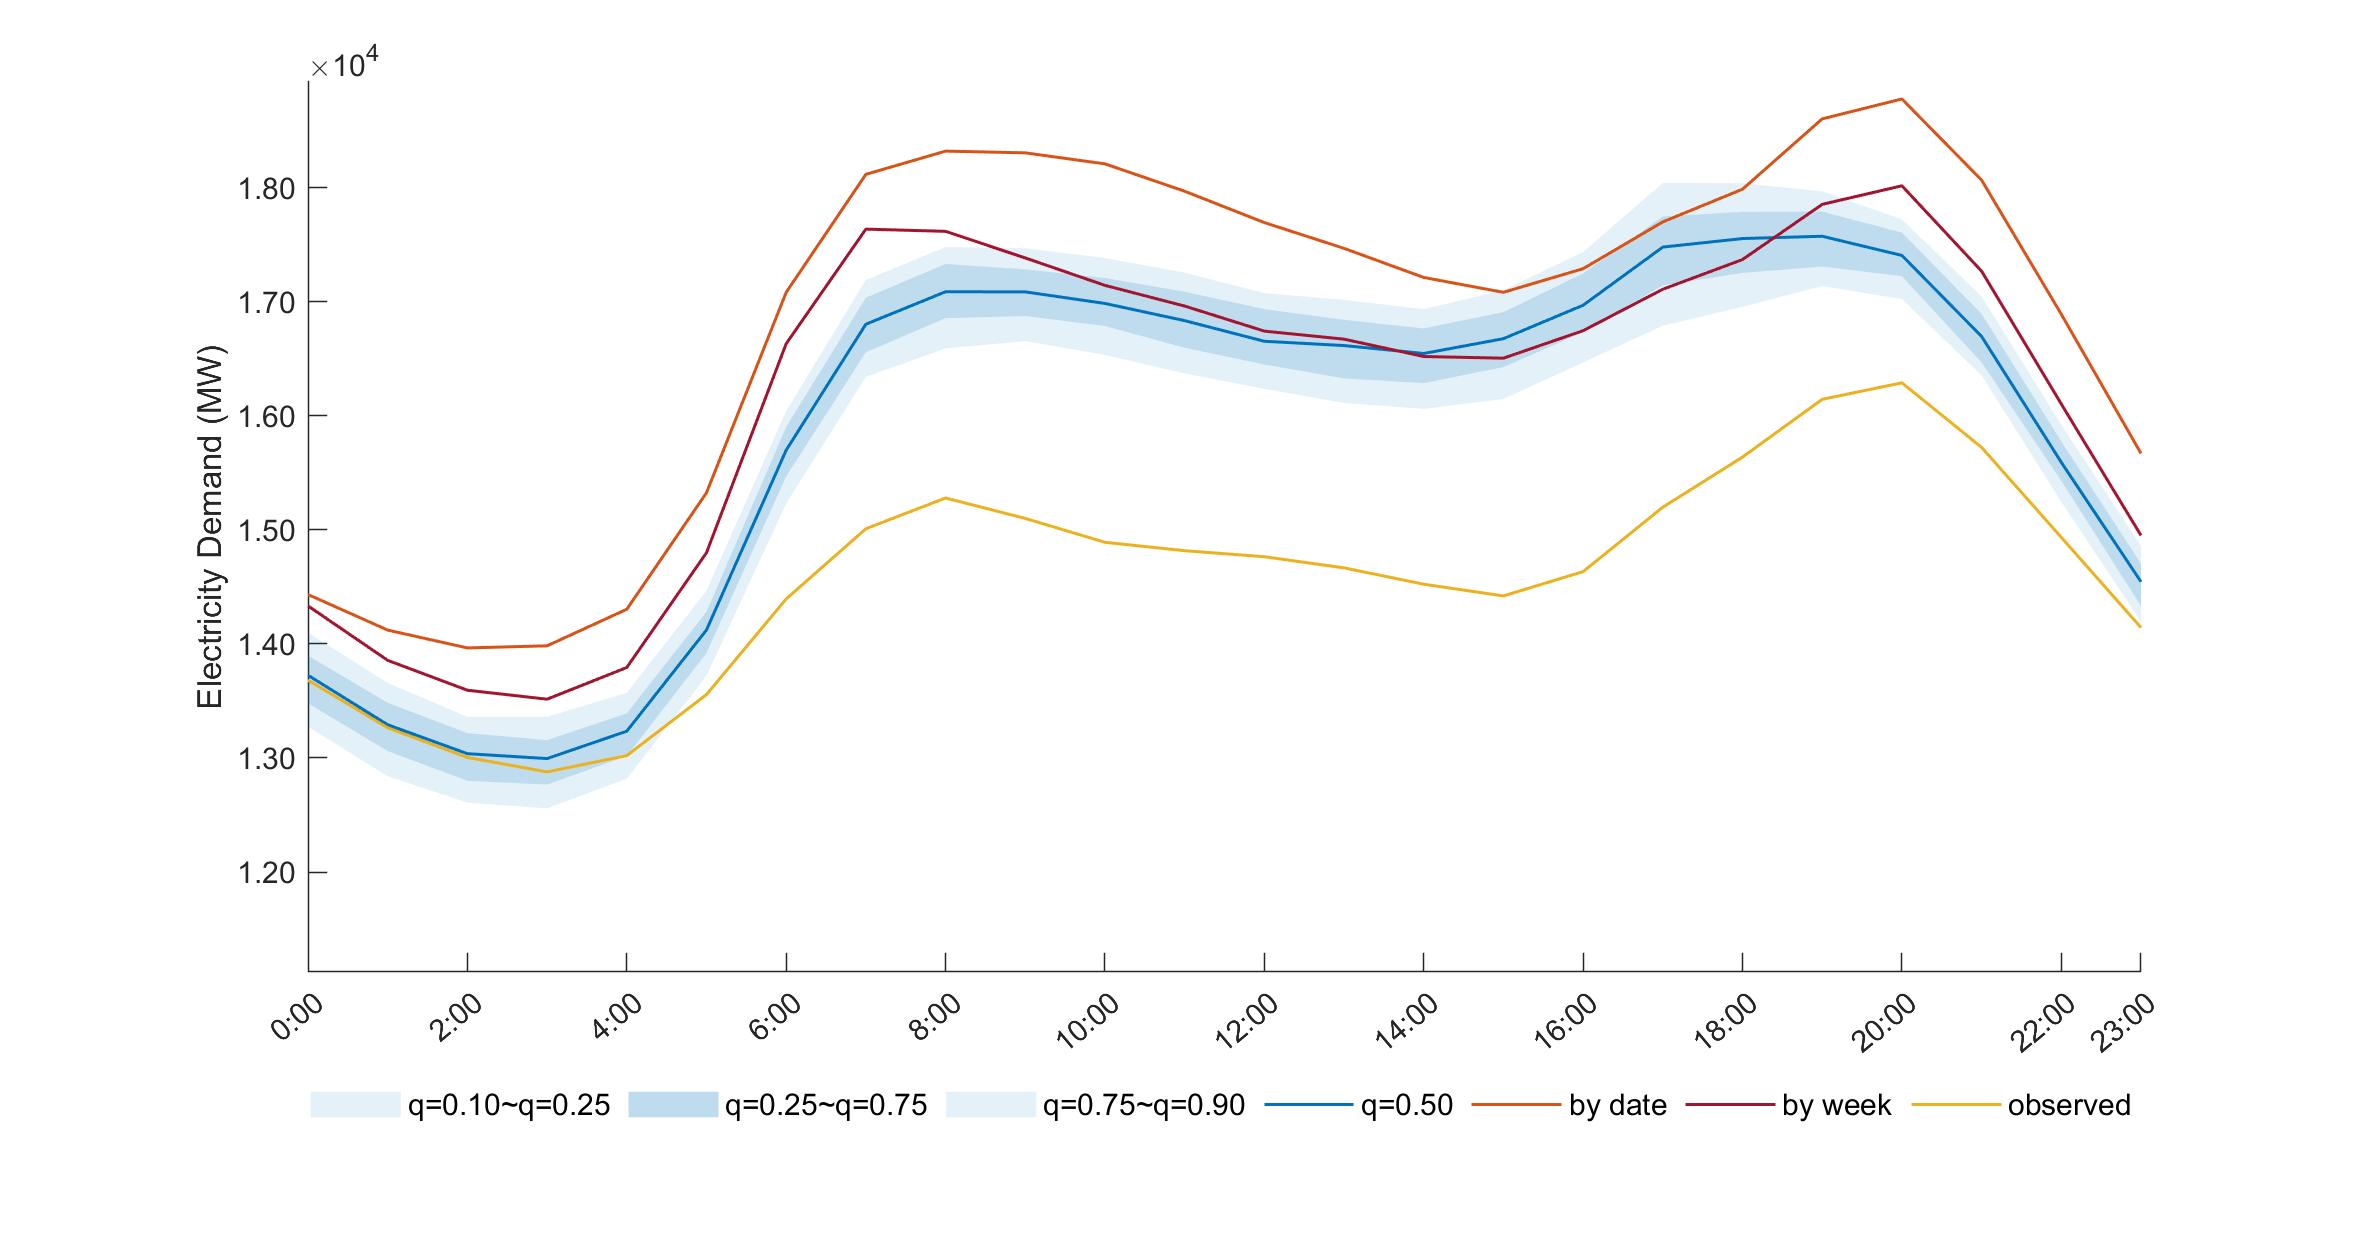
\includegraphics[width=0.8\textwidth]{figures/baseline_example1.jpg}
  \caption{Example: Baseline and Observed Demand of NYISO} \label{fig:baseline_eg1}
\end{figure}



%---------------------------------
\newpage
\section{Regression Analysis} \label{sec:regression}
 
To interpret the changes in electricity consumption during pandemic, three potential factors, namely, public health, social distancing, and the level of commercial activities, should be taken into account.In this section, we hereby introduce two regression methods to study the relationships between influential factors and electricity consumption.

Moreover, \covemda \quad supports regression based on any factors, including external data inputs. Users may define how the factors are regressed, including by linear, interaction, quadratic or pure-quadratic methods.

\subsection{OLS}\label{subsec:ols}

Ordinary least squares(OLS) models are implemented in \covemda. It includes linear and non-linear models and offers multiple choices for model fitting. Besides, \covemda \quad also support correlation analysis for variables either from COVID-EMDA+ or from external sources.

\begin{equation}
  min f(x)=\sum^{m}_{i=1}L_i^2(x)=\sum^{m}_{i=1}[y_i-f(x_i,\omega_i)]^2,
\end{equation}
Ordinary least squares aim for the minimum value of the formula above, in which $L_i(x)$ is the residual function. If $L_i(x)$ is a linear function about $x$, the optimization problem is called 'linear least squares problem', while nonlinear ones are addressed as 'nonlinear least squares problems'. 

\subsection{VAR}\label{subsec:var}


Restricted Vector Autoregression (Restricted VAR) models are implemented in \covemda as well. Restricted VAR models are powerful tools for multivariate time series analysis with complex correlations.

Vector autoregression (VAR)\cite{var} is a stochastic process model that can be used to capture the linear correlation between multiple time-series. We model the dynamics of reduction in electricity consumption using a Restricted VAR model of order p as follows:

\begin{equation}
  X_t=C+A_1X_{t-1}+\dots+A_pX_{t-p}+E_t,
\end{equation}
where
\begin{equation}
  A_i=
  \begin{bmatrix}
  a_{1,1}^i & a_{1,2}^i & \cdots & a_{1,n}^i\\
  a_{2,1}^i & a_{2,2}^i & \cdots & a_{2,n}^i\\
  \vdots & \vdots & \ddots & \vdots \\
  a_{n,1}^i & a_{n,2}^i & \cdots & a_{n,n}^i\\
  \end{bmatrix}
  ,X_t=
  \begin{bmatrix}
    x_t^1\\x_t^2\\\vdots\\x_t^n
  \end{bmatrix},
  C=
  \begin{bmatrix}
    c^1\\c^2\\\vdots\\c^n
  \end{bmatrix},
  E_t=
  \begin{bmatrix}
    e_t^1\\e_t^2\\\vdots\\e_t^n
  \end{bmatrix},
\end{equation}
in which $A_i$ is the regression matrix, $x_t^1$ represents the target output variable at time $t$, namely the reduction in electricity consumption we wish to model, $x_t^2,\cdots,x_t^n$ represent the selected $n-1$ parameter variables including confirmed case numbers, stay-at-home population, median home dwell time rate, population of on-site workers, mobility in the retail sector and etc., $C$ and $E_t$ are respectively column vectors of intercept and random errors, and the time notation $t-p$ represents the $p$-th lag of the variables.

The full procedure of building the restricted VAR model mainly contains four steps as follows, including pre-estimation preparation, restricted VAR model estimation, restricted VAR model verification, and post-estimation analysis.
\subsubsection{Pre-estimation Preparation}
\begin{itemize}
  \item Data Preprocessing: Several datasets are collected to calculate the inputs of restricted VAR model, including electricity market data, weather data, number of COVID-19 cases, and mobile device location data. We take logarithms of several variables, including electricity consumption reduction, new daily confirmed cases, stay-at-home population, population of full-time on-site workers, population of part-time on-site workers, and mobility in the retail sector, while only keeping the original value of the median home dwell time rate.
  \item Augmented Dickey-Fuller (ADF) Test: Test whether a time-series variable is non-stationary and possesses a unit root.
  \item Cointegration Test: Test the long-term correlation between multiple non-stationary time-series.
  \item Granger Causality Wald Test: Estimate the causality relationship among two variables represented as time-series.
\end{itemize}
\subsubsection{Restricted VAR Model Estimation}
\begin{itemize}
  \item  Ordinary Least Square (OLS): We impose constraints on the OLS to eliminate any undesirable causal relationships between variables.
\end{itemize}
\subsubsection{Restricted VAR Model Verification}
\begin{itemize}
  \item ADF Test: Verify if the residual time-series are non-stationary and possess a unit root.
  \item Ljung-Box Test: Verify the endogeneity of the residual data that may render the regression result untrustworthy.
  \item Durbin-Watson Test: Detect the presence of autocorrelation at log 1 in the residuals of the Restricted VAR model.
  \item Robustness Test: Test the robustness of the Restricted VAR model against parameter perturbations.
\end{itemize}
\subsubsection{Post-estimation Analysis}
\begin{itemize}
  \item Impulse Response Analysis: Describe the evolution of the Restricted VAR model’s variable in response to a shock in one or more variables.
  \item Forecast Error Variance Decomposition: Aid in the interpretation of the Restricted VAR model by determining the proportion of each variable’s forecast variance that is contributed by shocks to the other variables.
\end{itemize}


\subsection{Functions}\label{subsec:functions}

\subsubsection{\texttt{exchange\_columns}}\label{func:exchange_columns}

\begin{Code}
function output=exchange_columns(table,column1,column2)
\end{Code}

Function \verb!exchange_columns! provides a function for columns exchange in tables. The inputs includes the table to be operated, the number or title of the two columns to be exchanged. The output of this function is the new table whose columns have been exchanged.

\subsubsection{\texttt{OLS}}\label{func:OLS}\label{subsubsec:OLS}

\begin{Code}
function output=OLS(table,varnum,varargin)
\end{Code}

Function \verb!OLS! gives a solution to the regression model in Section~\ref{subsec:ols}. The output is a printed table containing regression vector and correlation analysis. All parameter names are listed in Table~\ref{tab:OLS}.

\begin{table}[!ht]
  \centering
  \begin{threeparttable}
    \caption{OLS Parameters and Options}
    \label{tab:OLS}
    \footnotesize
    \begin{tabular}{lp{.3\textwidth}p{0.5\textwidth}}
      \toprule
      Name & Type & Description \\
      \midrule
     table & input & Table of variable vectors for regression\\
           \midrule
     varnum & input & Numbers of input variable vectors\\
      \midrule
     output & vector & Regression results\\
      \midrule
      regression model & \begin{tabular}[t]{l}
    linear   \\
    interaction \\
    quadratic   \\
    purequadratic \\
      \end{tabular} &  
      \begin{tabular}[t]{l}
    Constant and linear terms  \\ 
    Constant, linear, and interaction terms  \\
    Constant, linear, interaction, and squared terms \\
    Constant, linear, and squared terms\\
      \end{tabular}\\
    & & \begin{tabular}[t]{l @{ -- } l}
        Default & \verb!'linear'!. \\
      \end{tabular}                         \\
      \bottomrule
    \end{tabular}
  \end{threeparttable}
\end{table}

\subsubsection{\texttt{VAR}}\label{func:VAR}\label{subsubsec:VAR}

\begin{Code}
function VAR(table,varnum,order)
\end{Code}

Function \verb!VAR! gives a solution to the regression model in Section~\ref{subsec:var}. The output is a printed table containing regression vector and correlation analysis. Unlike OLS regression model, VAR doesn't distinguish dependent variables and independent variables. It gives an evaluation table of the parameters, listing the coefficient values between each two variables. All parameter names are listed in Table~\ref{tab:OLS}.

\begin{table}[!ht]
  \centering
  \begin{threeparttable}
    \caption{VAR Parameters and Options}
    \label{tab:OLS}
    \footnotesize
    \begin{tabular}{lp{.3\textwidth}p{0.5\textwidth}}
      \toprule
      Name & Type & Description \\
      \midrule
     table & input & Table of variable vectors for regression\\
      \midrule
     varnum & input & Numbers of input variable vectors\\
      \midrule
     order & input & order of the VAR model\\                   
      \bottomrule
    \end{tabular}
  \end{threeparttable}
\end{table}

\subsection{Examples}\label{subsec:examples}

In this section, we introduce the usage of the functions above with several examples. It is recommended to use feature-oriented high-level functions (see \ref{subsec:func_list}), and the following explanations and instructions are designed for them.

All high-level functions mentioned above (\verb!OLS! and \verb!VAR!) have similar input forms and can be used similarly. To be specific, the first input argument (table name) is compulsory, and the basic operation function \verb!basic_read! can help import csv files in format of tables. 

\subsubsection{OLS example}\label{subsec:ols example}

As for function \verb!OLS!, choosing a regression model is an essential step. Four OLS models are provided as follows, with each formula introduced in Section~\ref{subsubsec:OLS}.
\begin{center}
  \verb!'linear' | 'interaction' | 'quadratic' | 'purequadratic'!
\end{center}

As introduced above in Section~\ref{subsubsec:OLS}, the feature-oriented high-level function \verb!OLS! takes form as follows:

\begin{Command}
OLS(table,varnum,varargin);
\end{Command}

Meanwhile, user may probably need basic-operation functions \verb!basic_read! and \verb!exchange_columns!, which take forms as follows:

\begin{Command}
t = basic_read(filename);
\end{Command}

\begin{Command}
output = exchange_columns(table,column1,column2)
\end{Command}

For example, if user needs to do a regression with data from \verb!Covid Emda+ Data Hub!: \verb!'caiso_la_patterns.csv'!, he may do some data-preprocessing before regression. Firstly, user may employ the basic-operation function \verb!basic_read! to import data in table format. Secondly, \verb!OLS! takes the fist column from table as dependent variables by default and the following columns as independent ones. Accordingly, function \verb!exchange_columns! should be applied to exchange columns of table. Last but not least, user may do the regression part. Code example is provided below:

\begin{Command}
>> t=basic_read('caiso_la_patterns')

t =

  329x4 table

       date       Restaurant_Recreaction    Grocery_Pharmacy      Retail  
    __________    ______________________    ________________    __________

    2019-12-30          3.2519e+05             1.0855e+05       6.1559e+05
    2019-12-31          3.1989e+05             1.0976e+05       5.8792e+05
    2020-01-01          2.3363e+05                  51943       3.6671e+05
    2020-01-02          2.9873e+05                  90239        5.481e+05
                ...                                     ...

>> t=exchange_columns(t,1,4)

t =

  329x4 table

      Retail      Restaurant_Recreaction    Grocery_Pharmacy       date   
    __________    ______________________    ________________    __________

    6.1559e+05          3.2519e+05             1.0855e+05       2019-12-30
    5.8792e+05          3.1989e+05             1.0976e+05       2019-12-31
    3.6671e+05          2.3363e+05                  51943       2020-01-01
     5.481e+05          2.9873e+05                  90239       2020-01-02
              ...                                     ...

>> b=OLS(t,3,'linear')
               OLS Regerssion Results 
====================================================
           Model:                      OLS
           Method:           Least Squares
           Date:      29-Jun-2021 11:59:42
           Time:                   0.392 s
           R-squared:                0.996
           Adj. R-squared:           0.996
           F-statistic:              38471.97
           Prob (F-statistic):     
====================================================
        coef        std err        t         P>|t|      
      -8028.9       1872.5      -4.2879   2.3789e-05
        1.207     0.018001       67.051  8.9386e-193
       2.0651     0.075663       27.294    3.344e-86


b =

      -8028.9
        1.207
       2.0651

\end{Command}


\subsubsection{VAR example}\label{subsec:var example}

As for function \verb!VAR!, the regression mode is already set. And as introduced above in Section~\ref{subsubsec:VAR}, the feature-oriented high-level function \verb!VAR! takes form as follows:

\begin{Code}
function VAR(table,varnum,order);
\end{Code}

Unlike function \verb!OLS!, there is no output for this function. Meanwhile, user may probably need basic-operation functions \verb!basic_read! and \verb!exchange_columns!, which take forms as follows:

\begin{Code}
function t = basic_read(filename);
\end{Code}

\begin{Code}
function output = exchange_columns(table,column1,column2)
\end{Code}

For example, if user needs to do a VAR with data from \verb!Covid Emda+ Data Hub!: \verb!'caiso_rto_lmp.csv'!, he may do some data-preprocessing before regression. Firstly, user may employ the basic-operation function \verb!basic_read! to import data in table format. 
\begin{Command}
>> t=basic_read('caiso_rto_lmp')

t =

  1462x25 table

       date       00:00     01:00     02:00             ...
    __________    ______    ______    ______            ...

    2017-01-19     21.53     21.69     20.86            ...
    2017-01-20     26.46     24.67     23.68            ...
    2017-01-21     30.83     28.37     28.19            ...
    2017-01-22     27.33     26.5      25.14            ...
                ...                  ...                ...
\end{Command}

Secondly, \verb!VAR! takes the fist few columns from table as variables by default, and the other columns remain untouched. Accordingly, function \verb!exchange_columns! should be applied to exchange columns of table. 
\begin{Command}
>> t=exchange_columns(t,1,4)

t =

  1462x25 table

    02:00     00:00     01:00        date    
    ______    ______    ______    __________            ...

    20.86     21.53     21.69     2017-01-19            ...
    23.68     26.46     24.67     2017-01-20            ...
    28.19     30.83     28.37     2017-01-21            ...
    25.14     27.33     26.5      2017-01-22            ...
            ...                  ...                    ...
\end{Command}

Last but not least, user may do the VAR part. 
\begin{Command}
>> VAR(t,3,2)
               OLS Regerssion Results 
====================================================
           Model:                      VAR
           Method:           Least Squares
           Date:      29-Jun-2021 16:06:28
====================================================
        coef        std err         t         P>|t|     
       2.2366       0.3111       7.1893   1.0376e-12
      0.85631     0.087143       9.8265   4.1469e-22
    -0.073503     0.064774      -1.1348      0.25666
      0.16578      0.11112       1.4919      0.13594
    -0.024319     0.087911     -0.27663       0.7821
    -0.052469     0.064236     -0.81681      0.41417
     0.051594       0.1113      0.46356      0.64304
%% each sub table have 3x2+1=7 rows

        coef        std err         t         P>|t|     
       2.8308       0.3498       8.0927   1.2202e-15
       0.3993     0.097985       4.0751    4.847e-05
      0.31999     0.072833       4.3934   1.1966e-05
       0.2698      0.12494       2.1594     0.030985
      -0.1529     0.098849      -1.5468      0.12213
      0.13715     0.072228       1.8989     0.057782
    -0.025913      0.12515     -0.20706      0.83599


        coef        std err         t         P>|t|     
       2.6695      0.32137       8.3065   2.2288e-16
      0.57071     0.090021       6.3398   3.0629e-10
     0.031848     0.066913      0.47596      0.63417
      0.36905      0.11479        3.215    0.0013332
    -0.085903     0.090815     -0.94591      0.34435
    -0.022497     0.066357     -0.33903      0.73463
     0.064468      0.11498      0.56071      0.57508
\end{Command}


%--------------------------------------------
\newpage
\section{Visualization} \label{sec:visual}

\subsection{Generation Mix}

After the COVID-19 outbreak, the total generation as well as generation share of each market in U.S. varied. In order to analyse this change, we may observe the generation data in scale of time or of generation fuels. This may offer a new approach for researchers to find out the structure change of U.S. power grid brought by COVID-19.

In \covemda{}, two typical tools regarding different scales are provided for generation analysis: \verb!plot_generation_mix! and \verb!plot_renewable_share!. Function \verb!plot_generation_mix! plots the generation mix data in the form of filled areas, and function \verb!plot_renewable_share! plots the renewable share data in the form of a line chart. Both of them obtain relevant data from file \verb!<market_name>_rto_genmix.csv! in the data hub. See Section~\ref{func:plot_generation_mix} and Section~\ref{func:plot_renewable_share} for more detail.

\begin{Command}
>> plot_generation_mix('spp');
\end{Command}

\begin{figure}[ht]
  \centering
  \noindent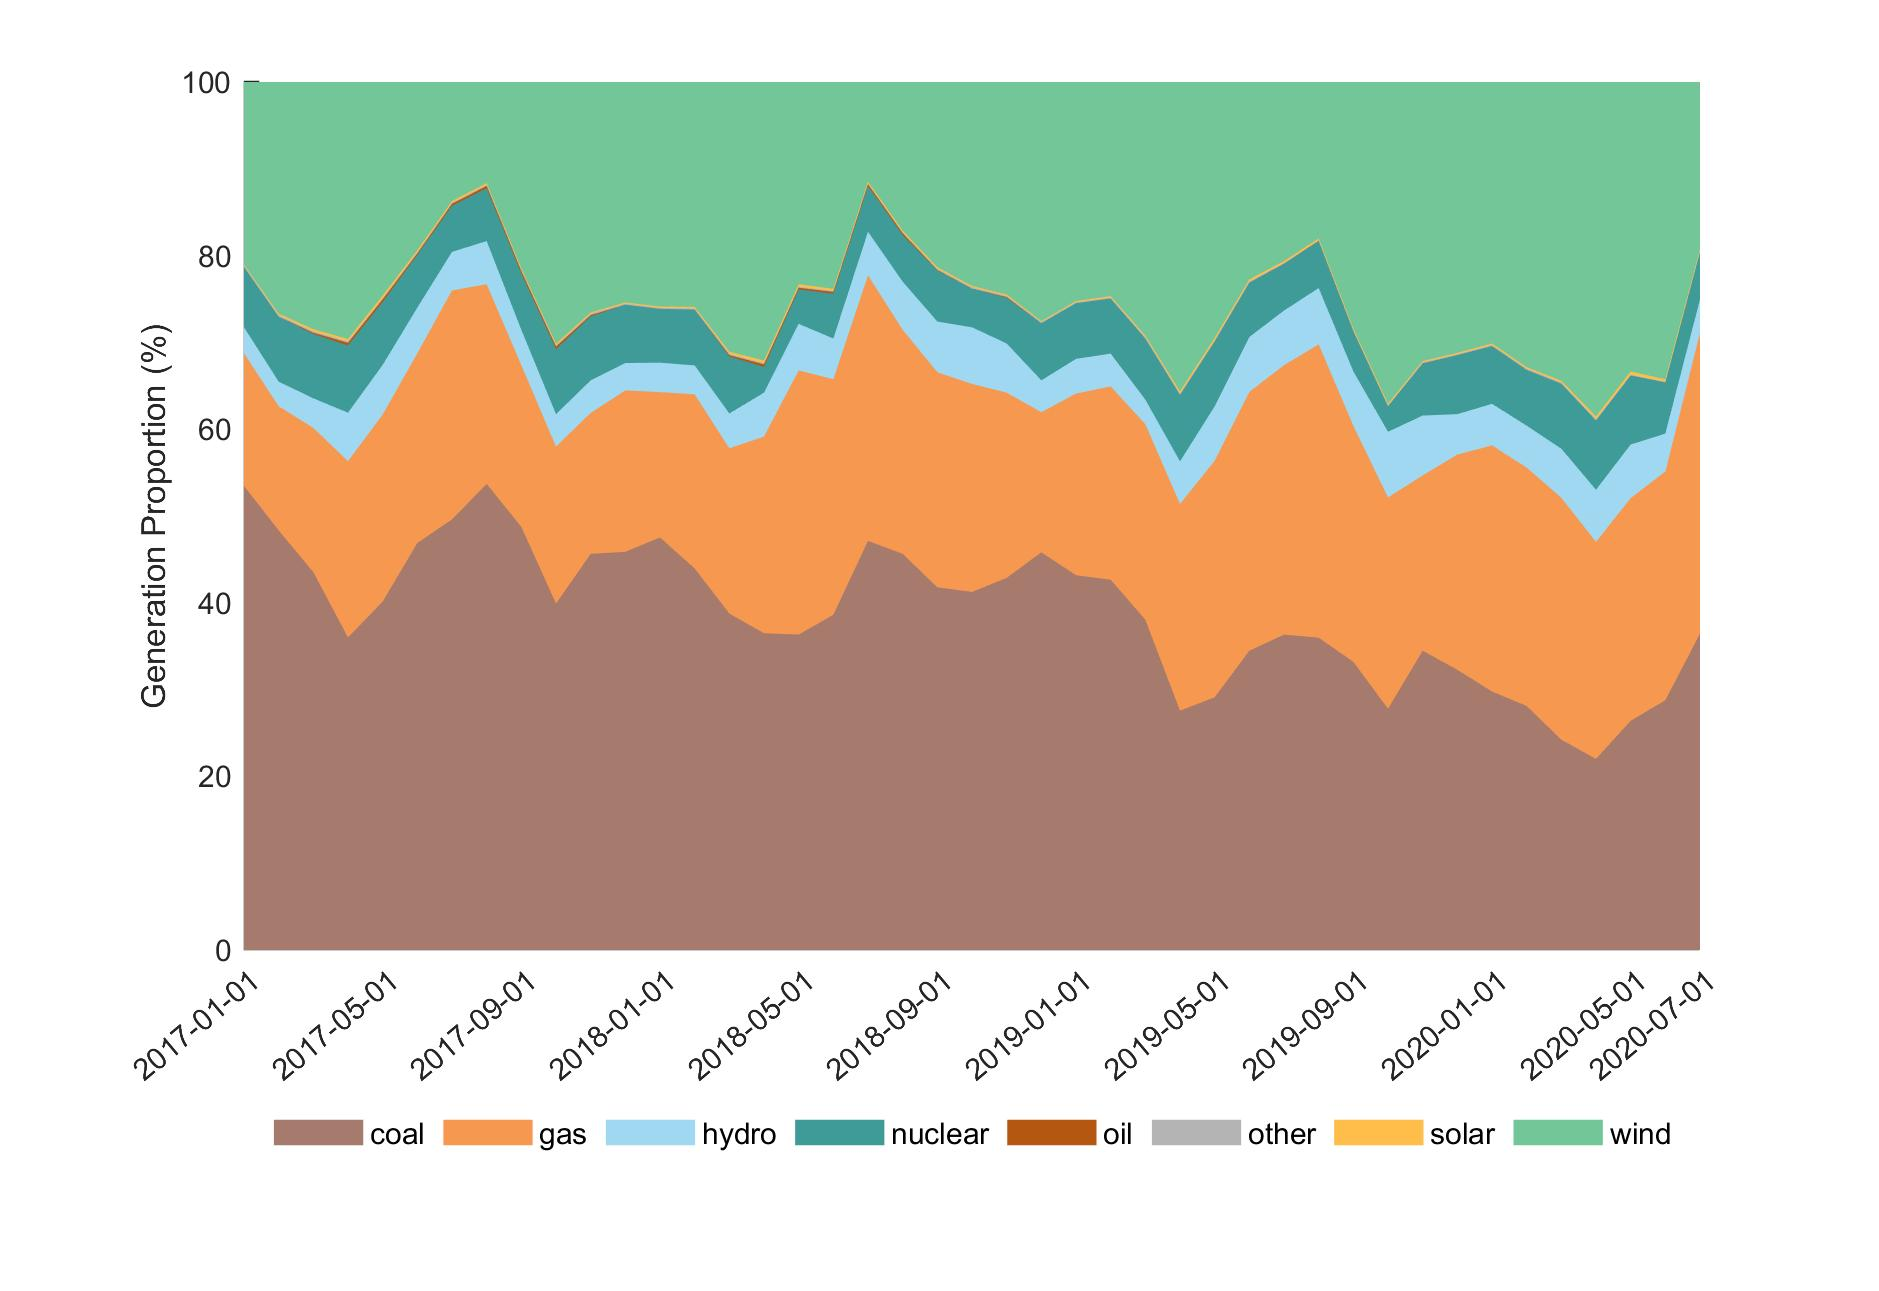
\includegraphics[width=0.8\textwidth]{figures/visualization_plot_generation_mix.jpg}
  \caption{Generation Mix of SPP} \label{fig:vis_1}
\end{figure}

One possible output of function \verb!plot_generation_mix! with default settings is displayed in Figure~\ref{fig:vis_1}. Different color blocks demonstrate different fuel kinds as shown in legends. The area of each block shows the electric generation of each kind of fuel. In this figure, we may see that the main generation structure change is caused by the quantity of wind power generation.



\subsection{Demand Profiles}

Electric power demand is a significant aspect of power system analysis. After the COVID-19 outbreak, the features of demand profiles across all U.S. electricity markets have experienced several changes, which offer the researchers an important perspective to analyze the relationship between the pandemic, electricity demand patterns and power system operation.

In \covemda{}, two typical tools regarding different time scales are provided for demand analysis: \verb!plot_demand! and \verb!plot_daily_demand_curve!. Function \verb!plot_demand! plots the load data in the form of a line chart, and function \verb!plot_daily_demand_curve! plots the demand distribution curve in the form of multiple areas. Both of them obtain relevant data from file \verb!<market_name>_<city_name>_load.csv! in the data hub. See Section~\ref{func:plot_demand} and Section~\ref{func:plot_daily_demand_curve} for more detail.

\begin{Command}
>> plot_daily_demand_curve('nyiso');
\end{Command}

\begin{figure}
  \centering
  \noindent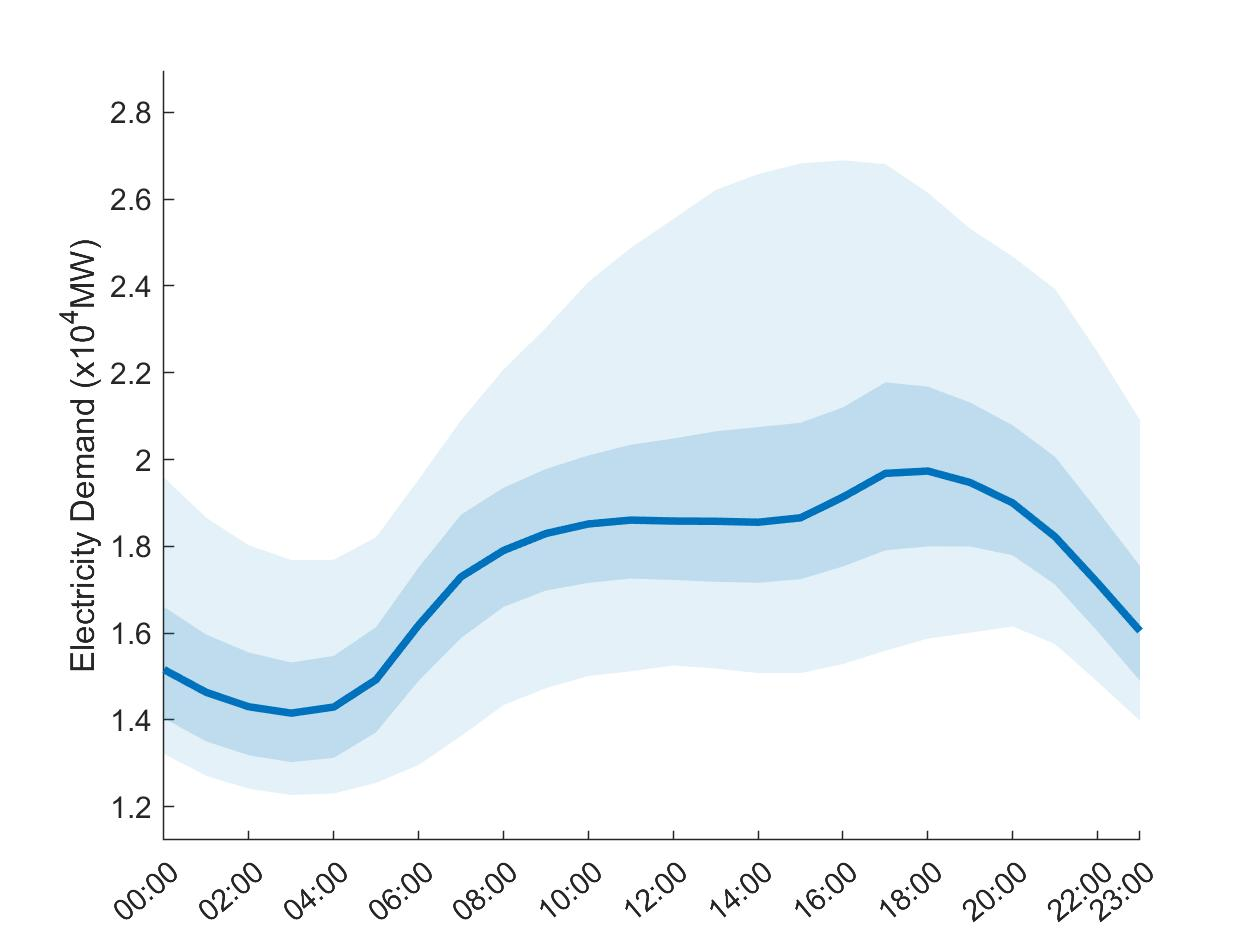
\includegraphics[width=0.8\textwidth]{figures/visualization_plot_daily_demand_curve.jpg}
  \caption{Daily Demand Curve of NYISO} \label{fig:vis_1}
\end{figure}

One possible output of function \verb!plot_daily_demand_curve! with default settings is displayed in Figure~\ref{fig:vis_1}. In this plot, five edges of color blocks represent the five quantiles, \verb![0.05, 0.25, 0.5, 0.75, 0.95]! successively. As there are odd quantiles, the \verb!0.5! quantile is displayed as the central line. The outer light blue area represents the variation of \verb!0.05~0.95!, and the inner less-light blue area represents \verb!0.25~0.75!, to better illustrate the variation of electricity demand in the date range.



\subsection{Price Distribution}

In this section, we provide two typical tools to display the electricity price in U.S. After the COVID-19 outbreak, electricity price become harder to trace. In order to trace the change of electricity price, we may observe the price data of different markets in U.S. and organize them into plots. This may offer a new approach for researchers to find out the structure change of U.S. power grid brought by COVID-19.

In \covemda{}, two typical tools regarding different scales are provided for price analysis: \verb!plot_price! and \verb!plot_price_distribution!. Function \verb!plot_price! plots the price data in the form of a line chart, and function \verb!plot_price_distribution! plots the price distribution in the form of a histogram. Both of them obtain relevant data from file \\\verb!<market_name>_<city_name>_lmp.csv! in the data hub. See Section~\ref{func:plot_price} and Section~\ref{func:plot_price_distribution} for more detail.



\subsection{Mobility}

Mobility is a factor directly related with the pandemic. Here 'mobility' means the number of visits to business premises, indicating the level of commercial activities. During COVID-19, the mobility in various sectors have experienced dramatic reduction, which is one of the first signals of the outbreak.

In \covemda{}, the mobility data for three sectors are provided: \verb!Restaurant_Recreation!, \verb!Grocery_Pharmacy! and \verb!Retail!. Unlike other functions in this section, here the data are focused on \textbf{seven major cities}: Los Angeles(\verb!la!), Houston(\verb!houston!), Boston(\verb!boston!), New York City(\verb!nyc!), Chicago(\verb!chicago!), Philadelphia(\verb!phila!) and Kansas City(\verb!kck!). All the data above are obtained from file \verb!<market_name>_<city_name>_patterns.csv! and can be visualized by function \verb!plot_mobility!. See Section~\ref{func:plot_mobility} for more detail.



\subsection{Functions}

\subsubsection{\texttt{plot\_generation\_mix}}\label{func:plot_generation_mix}

\begin{Code}
function ar=plot_generation_mix(market,varargin)
\end{Code}

Function \verb!plot_generation_mix! plots the generation mix of a market within specified date range. Like \verb!area!, it returns the area objects of the curve for further modification. This function is based on \matlab{} function \verb!area!.

By default, this function plots the generation mix of the specified market from 2017-01-01 to 2020-07-15 with month resampling. Additional name-value pair arguments are available for modifications. See Table~\ref{tab:plot_generation_mix} for a full list of arguments.

\begin{table}[!ht]
\centering
\begin{threeparttable}
\caption{Plot Generation Mix Options}
\label{tab:plot_generation_mix}
\footnotesize
\begin{tabular}{lp{.3\textwidth}p{0.5\textwidth}}
\toprule
Name & Type & Description \\
\midrule
DateRange & \begin{tabular}[t]{l}
datetime array\\
string array\\
cell array of character vectors\\
\end{tabular} & Range of time. \\
& & \begin{tabular}[t]{l @{ -- } l}
Default & \verb!{'2017-01-01','2020-07-15'}!.\\
Example & \verb!{'2017-01-01','2020-07-15'}!\\
& \verb!["2020-02-01","2020-04-30"]!\\
\end{tabular}\\
\midrule
      City & \begin{tabular}[t]{l}
        string    \\
        character array \\
      \end{tabular} & Abbreviation of the target city or \verb!'rto'! for the entire market.  \\
       & & \begin{tabular}[t]{l @{ -- } l}
        Default & \verb!'rto'!. \\
      \end{tabular}                         \\
\midrule
ResampleBin & \begin{tabular}[t]{l}
string\\
character vectors\\
\end{tabular} & Binning scheme for resampling.\\
& & \begin{tabular}[t]{l @{ -- } l}
Default & \verb!'month'!.\\
\end{tabular}\\
\midrule
Others & & See Section~\ref{func:plot_area}.\\
\bottomrule
\end{tabular}
\end{threeparttable}
\end{table}



\subsubsection{\texttt{plot\_renewable\_share}}\label{func:plot_renewable_share}

\begin{Code}
function p=plot_renewable_share(market,varargin)
\end{Code}

Function \verb!plot_renewable_share! plots the renewable share curve of a market within specified date range. Like \verb!plot!, it returns the line objects of the curve for further modification. This function is based on \matlab{} function \verb!plot!.

By default, this function plots the renewable share of the specified market from 2017-01-01 to 2020-07-15, with no resampling. Additional name-value pair arguments are available for modifications. See Table~\ref{tab:plot_renewable_share} for a full list of arguments.

\begin{table}[!ht]
\centering
\begin{threeparttable}
\caption{Plot Renewable Share, Plot Demand and Plot Price Options}
\label{tab:plot_renewable_share}
\footnotesize
\begin{tabular}{lp{.3\textwidth}p{0.5\textwidth}}
\toprule
Name & Type & Description \\
\midrule
DateRange & \begin{tabular}[t]{l}
datetime array\\
string array\\
cell array of character vectors\\
\end{tabular} & Range of time. \\
& & \begin{tabular}[t]{l @{ -- } l}
Default & \verb!{'2017-01-01','2020-07-15'}!.\\
Example & \verb!{'2017-01-01','2020-07-15'}!\\
& \verb!["2020-02-01","2020-04-30"]!\\
\end{tabular}\\
\midrule
      City & \begin{tabular}[t]{l}
        string    \\
        character array \\
      \end{tabular} & Abbreviation of the target city or \verb!'rto'! for the entire market.  \\
       & & \begin{tabular}[t]{l @{ -- } l}
        Default & \verb!'rto'!. \\
      \end{tabular}                         \\
\midrule
ResampleBin & \begin{tabular}[t]{l}
string\\
character vectors\\
\end{tabular} & Binning scheme for resampling. \\
& & \begin{tabular}[t]{l @{ -- } l}
Default & \verb!'none'!.\\
\end{tabular}\\
\midrule
      ResampleMethod & \begin{tabular}[t]{l}
        string            \\
        character vectors \\
      \end{tabular} & Computation method for resampling. \tnote{\dag}        \\
                  &                            & \begin{tabular}[t]{l @{ -- } l}
        Default & \verb!'mean'!. \\
      \end{tabular}                         \\
      \midrule
Others & & See Section~\ref{func:plot_line_chart}.\\
\bottomrule
\end{tabular}
\end{threeparttable}
\end{table}



\subsubsection{\texttt{plot\_demand}}\label{func:plot_demand}

\begin{Code}
function p=plot_demand(market,varargin)
\end{Code}

Function \verb!plot_demand! plots the demand curve of a market within specified date range. Like \verb!plot!, it returns the line object of the curve for further modification. This function is based on \matlab{} function \verb!plot!.

By default, this function plots the demand curve of the specified market from 2017-01-01 to 2020-07-15, with no resampling. Additional name-value pair arguments are available for modifications. See Table~\ref{tab:plot_renewable_share} for a full list of arguments.



\subsubsection{\texttt{plot\_daily\_demand\_curve}}\label{func:plot_daily_demand_curve}

\begin{Code}
function gr_handles=plot_daily_demand_curve(market,varargin)
\end{Code}

Function \verb!plot_daily_demand_curve! plots the daily demand curve of a market with specified quantiles. It returns all the objects in the plot for further modification. If there are odd quantiles, the central one is displayed as a line object. Otherwise all of them are displayed as area objects. This function is based on \matlab{} function \verb!area! and \verb!plot!.

By default, this function plots the daily demand curve of the specified market from 2017-01-01 to 2020-07-15 with the five quantiles representing its variation: \verb![0.05, 0.25, 0.5, 0.75, 0.95]!. Additional name-value pair arguments are available for modifications. See Table~\ref{tab:plot_daily_demand_curve} for a full list of arguments.

\begin{table}[!ht]
  \centering
  \begin{threeparttable}
    \caption{Plot Daily Demand Curve Options}
    \label{tab:plot_daily_demand_curve}
    \footnotesize
    \begin{tabular}{lp{.3\textwidth}p{0.5\textwidth}}
      \toprule
      Name        & Type                       & Description                                        \\
      \midrule
      DateRange   & \begin{tabular}[t]{l}
        datetime array                  \\
        string array                    \\
        cell array of character vectors \\
      \end{tabular} & Range of time.                                     \\
                  &                            & \begin{tabular}[t]{l @{ -- } l}
        Default & \verb!{'2017-01-01','2020-07-15'}!. \\
        Example & \verb!{'2017-01-01','2020-07-15'}!  \\
                & \verb!["2020-02-01","2020-04-30"]!  \\
      \end{tabular}                         \\
      \midrule
      City & \begin{tabular}[t]{l}
        string    \\
        character array \\
      \end{tabular} & Abbreviation of the target city or \verb!'rto'! for the entire market.  \\
       & & \begin{tabular}[t]{l @{ -- } l}
        Default & \verb!'rto'!. \\
      \end{tabular}                         \\
      \midrule
      Quantile   & \begin{tabular}[t]{l}
        numeric vector                  \\
      \end{tabular} & Cumulative probabilities. \\
                  &                            & \begin{tabular}[t]{l @{ -- } l}
        Default & \verb![0.05, 0.25, 0.5, 0.75, 0.95]!. \\
      \end{tabular}                         \\
      \midrule
      Others & & See Section~\ref{func:plot_quantile}.\\
      \bottomrule
    \end{tabular}
  \end{threeparttable}
\end{table}



\subsubsection{\texttt{plot\_price}}\label{func:plot_price}

\begin{Code}
function p=plot_price(market,varargin)
\end{Code}

Function \verb!plot_price! plots the price curve of a market within specified date range. Like \verb!plot!, it returns the line objects of the curve for further modification. This function is based on \matlab{} function \verb!plot!.

By default, this function plots the price of the specified market from 2017-01-01 to 2020-07-15, with no resampling. Additional name-value pair arguments are available for modifications. See Table~\ref{tab:plot_renewable_share} for a full list of arguments.



\subsubsection{\texttt{plot\_price\_distribution}}\label{func:plot_price_distribution}

\begin{Code}
function H=plot_price_distribution(market,varargin)
\end{Code}

Function \verb!plot_price_distribution! plots the price distribution of a market. This function is based on \matlab{} function \verb!plot!.

By default, this function plots the price distribution of the specified market from 2017-01-01 to 2020-07-15. Additional name-value pair arguments are available for modifications. See Table~\ref{tab:plot_price_distribution} for a full list of arguments.

\begin{table}[!ht]
  \centering
  \begin{threeparttable}
    \caption{Plot Price Distribution Options}
    \label{tab:plot_price_distribution}
    \footnotesize
    \begin{tabular}{lp{.3\textwidth}p{0.5\textwidth}}
      \toprule
      Name        & Type                       & Description                                        \\
      \midrule
      DateRange   & \begin{tabular}[t]{l}
        datetime array                  \\
        string array                    \\
        cell array of character vectors \\
      \end{tabular} & Range of time.                                     \\
                  &                            & \begin{tabular}[t]{l @{ -- } l}
        Default & \verb!{'2017-01-01','2020-07-15'}!. \\
        Example & \verb!{'2017-01-01','2020-07-15'}!  \\
                & \verb!["2020-02-01","2020-04-30"]!  \\
      \end{tabular}                         \\
      \midrule
      City & \begin{tabular}[t]{l}
        string    \\
        character array \\
      \end{tabular} & Abbreviation of the target city or \verb!'rto'! for the entire market.  \\
       & & \begin{tabular}[t]{l @{ -- } l}
        Default & \verb!'rto'!. \\
      \end{tabular}                         \\
      \midrule
      Others & & See Section~\ref{func:plot_histogram}.\\
      \bottomrule
    \end{tabular}
  \end{threeparttable}
\end{table}



\subsubsection{\texttt{plot\_mobility}}\label{func:plot_mobility}

\begin{Code}
function p=plot_mobility(market,varargin)
\end{Code}

Function \verb!plot_mobility! plots the appointed mobility curve of one of the seven cities. Like \verb!plot!, it returns the line object of the curve for further modification. This function is based on \matlab{} function \verb!plot!.

By default, this function plots the mobility data of the retail sector in the specified city from 2019-12-30 to 2020-11-22, with no resampling. Additional name-value pair arguments are available for modifications. See Table~\ref{tab:plot_mobility} for a full list of arguments.

\begin{table}[!ht]
  \centering
  \begin{threeparttable}
    \caption{Plot Mobility Options}
    \label{tab:plot_mobility}
    \footnotesize
    \begin{tabular}{lp{.3\textwidth}p{0.5\textwidth}}
      \toprule
      Name        & Type                       & Description                                        \\
      \midrule
      DateRange   & \begin{tabular}[t]{l}
        datetime array                  \\
        string array                    \\
        cell array of character vectors \\
      \end{tabular} & Range of time.                                     \\
                  &                            & \begin{tabular}[t]{l @{ -- } l}
        Default & \verb!{'2017-01-01','2020-07-15'}!. \\
        Example & \verb!{'2017-01-01','2020-07-15'}!  \\
                & \verb!["2020-02-01","2020-04-30"]!  \\
      \end{tabular}                         \\
      \midrule
      City & \begin{tabular}[t]{l}
        string    \\
        character array \\
      \end{tabular} & Abbreviation of the target city.  \\
       & & \begin{tabular}[t]{l @{ -- } l}
        Default & Corresponding city of the specified market. \\
      \end{tabular}                         \\
      \midrule
      Sector & \begin{tabular}[t]{l}
        string            \\
        character vectors \\
      \end{tabular} & The sector to be plotted. Can be assigned as \verb!'Retail'!, \verb!'Restaurant_Recreaction'! or \verb!'Grocery_Pharmacy'!.    \\
                  &                            & \begin{tabular}[t]{l @{ -- } l}
        Default & \verb!'Retail'!. \\
      \end{tabular}                         \\
      \midrule
      ResampleBin & \begin{tabular}[t]{l}
        string            \\
        character vectors \\
      \end{tabular} & Binning scheme for resampling. \\
                  &                            & \begin{tabular}[t]{l @{ -- } l}
        Default & \verb!'none'!. \\
      \end{tabular}                         \\
      \midrule
      ResampleMethod & \begin{tabular}[t]{l}
        string            \\
        character vectors \\
      \end{tabular} & Computation method for resampling. \\
                  &                            & \begin{tabular}[t]{l @{ -- } l}
        Default & \verb!'mean'!. \\
      \end{tabular}                         \\
      \midrule
      Others & & See Section~\ref{func:plot_line_chart}.\\
      \bottomrule
    \end{tabular}
  \end{threeparttable}
\end{table}



\subsubsection{\texttt{plot\_area}}\label{func:plot_area}

\begin{Code}
function ar=plot_area(t,varargin)
\end{Code}

Function \verb!plot_area! is the subfunction of \verb!plot_generation_mix!. As the modification of \matlab{} function \verb!area!, several default settings are altered for appearance. The first column of table \verb!t! is appointed as labels of the x-axis, and all the other columns contain data to be plotted. See Table~\ref{tab:plot_area} for a full list of arguments.

\begin{table}[!ht]
\centering
\begin{threeparttable}
\caption{Plot Area Options}
\label{tab:plot_area}
\footnotesize
\begin{tabular}{lp{.3\textwidth}p{0.5\textwidth}}
\toprule
Name & Type & Description \\
\midrule
      EdgeColor & \begin{tabular}[t]{l}
        RGB triplet \\
        hexadecimal color code \dots
      \end{tabular} & Color of the edges.  \\
       & & \begin{tabular}[t]{l @{ -- } l}
        Default & \verb!'none'!. \\
      \end{tabular}                         \\
\midrule
ColorMap & \begin{tabular}[t]{l}
table\\
structure array\\
string array\\
cell array of character vectors\\
\end{tabular} & Colors of all the areas in the plot. \\
& & \begin{tabular}[t]{l}
Default --\\
\verb!["coal","gas","oil","nuclear","hydro",!\\
\verb!"wind","solar","other","import";!\\
\verb!"#a67a6d","#f69850","#b35711","#3f9b98",!\\
\verb!"#a0d8f1","#73c698","#ffbd4a",!\\
\verb!"#b4b4b4","white"]!\\
\end{tabular}\\
\bottomrule
\end{tabular}
\end{threeparttable}
\end{table}



\subsubsection{\texttt{plot\_line\_chart}}\label{func:plot_line_chart}

\begin{Code}
function p=plot_line_chart(t,varargin)
\end{Code}

Function \verb!plot_line_chart! is the subfunction of \verb!plot_demand!, \verb!plot_mobility!, \verb!plot_price! and \verb!plot_renewable_share!. As the modification of \matlab{} function \verb!plot!, several default settings are altered for appearance. The first column of table \verb!t! is appointed as labels of the x-axis, and the second column contains data to be plotted. See Table~\ref{tab:plot_line_chart} for a full list of arguments.

\begin{table}[!ht]
\centering
\begin{threeparttable}
\caption{Plot Line Chart Options}
\label{tab:plot_line_chart}
\footnotesize
\begin{tabular}{lp{.3\textwidth}p{0.5\textwidth}}
\toprule
Name & Type & Description \\
\midrule
      DisplayName & \begin{tabular}[t]{l}
        string    \\
        character array \\
      \end{tabular} & Name (legend) to be displayed on the graph.  \\
       & & \begin{tabular}[t]{l @{ -- } l}
        Default & Name of the table column. \\
      \end{tabular}                         \\
      \midrule
      Color & \begin{tabular}[t]{l}
        RGB triplet \\
        hexadecimal color code \dots  \\
      \end{tabular} & Color of the line.        \\
                  &                            & \begin{tabular}[t]{l @{ -- } l}
        Default & \verb!'#0072BD'!. \\
      \end{tabular}                         \\
      \midrule
      LineWidth & positive numeric value & Width of the line.  \\
       & & \begin{tabular}[t]{l @{ -- } l}
        Default & \verb!1!. \\
      \end{tabular}                         \\
      \midrule
      LineStyle & character value & Style of the line.  \\
       & & \begin{tabular}[t]{l @{ -- } l}
        Default & \verb!'-'!. \\
      \end{tabular}                         \\
      \midrule
      Marker & character value & Style of the marker.  \\
       & & \begin{tabular}[t]{l @{ -- } l}
        Default & \verb!'none'!. \\
      \end{tabular}                         \\
\bottomrule
\end{tabular}
\end{threeparttable}
\end{table}



\subsubsection{\texttt{plot\_quantile}}\label{func:plot_quantile}

\begin{Code}
function gr_handles=plot_quantile(t,varargin)
\end{Code}

Function \verb!plot_quantile! is the subfunction of \verb!plot_daily_demand_curve!. The intervals are represented with areas of different brightness, indicating the distribution. The first column of table \verb!t! is appointed as labels of the x-axis, and the rest columns contain quantiles to be plotted. See Table~\ref{tab:plot_quantile} for a full list of arguments.

\begin{table}[!ht]
  \centering
  \begin{threeparttable}
    \caption{Plot Quantile Options}
    \label{tab:plot_quantile}
    \footnotesize
    \begin{tabular}{lp{.3\textwidth}p{0.5\textwidth}}
      \toprule
      Name        & Type                       & Description                                        \\
      \midrule
      Color & \begin{tabular}[t]{l}
        RGB triplet \\
        hexadecimal color code \dots  \\
      \end{tabular} & Color theme of the plot.        \\
                  &                            & \begin{tabular}[t]{l @{ -- } l}
        Default & \verb!'#0072BD'!. \\
      \end{tabular}                         \\
      \midrule
      Alpha & \begin{tabular}[t]{l}
        numeric vector            \\
      \end{tabular} & Face transparency of the objects.        \\
                  &                            & \begin{tabular}[t]{l @{ -- } l}
        Default & \verb![0.1, 0.25]!. \\
      \end{tabular}                         \\
      \midrule
      LineWidth & \begin{tabular}[t]{l}
        positive value            \\
      \end{tabular} & Width of the central line (if exists).       \\
                  &                            & \begin{tabular}[t]{l @{ -- } l}
        Default & \verb!1!. \\
      \end{tabular}                         \\
      \bottomrule
    \end{tabular}
  \end{threeparttable}
\end{table}



\subsubsection{\texttt{plot\_histogram}}\label{func:plot_histogram}

\begin{Code}
function h=plot_histogram(t,varargin)
\end{Code}

Function \verb!plot_histogram! is the subfunction of \verb!plot_price_distribution!. As the modification of \matlab{} function \verb!histogram!, several default settings are altered for appearance. The first column of table \verb!t! is appointed as labels of the x-axis, and the second column contains data to be plotted. See Table~\ref{tab:plot_histogram} for a full list of arguments.

\begin{table}[!ht]
  \centering
  \begin{threeparttable}
    \caption{Plot Histogram Options}
    \label{tab:plot_histogram}
    \footnotesize
    \begin{tabular}{lp{.3\textwidth}p{0.5\textwidth}}
      \toprule
      Name        & Type                       & Description                                        \\
      \midrule
      DisplayName & \begin{tabular}[t]{l}
        string    \\
        character array \\
      \end{tabular} & Name (legend) to be displayed on the graph.  \\
       & & \begin{tabular}[t]{l @{ -- } l}
        Default & Name of the table column. \\
      \end{tabular}                         \\
      \midrule
      Normalization & \begin{tabular}[t]{l}
        string    \\
        character array \\
      \end{tabular} & Method for data normalization. Can be assigned as \verb!'count'!, \verb!'probability'!, \verb!'countdensity'!, \verb!'pdf'!, \verb!'cumcount'! or \verb!'cdf'!.  \\
       & & \begin{tabular}[t]{l @{ -- } l}
        Default & \verb!'pdf'!. \\
      \end{tabular}                         \\
      \midrule
      EdgeColor & \begin{tabular}[t]{l}
        RGB triplet \\
        hexadecimal color code \dots
      \end{tabular} & Color of the edges.  \\
       & & \begin{tabular}[t]{l @{ -- } l}
        Default & \verb!'none'!. \\
      \end{tabular}                         \\
      \midrule
      NumBins & \begin{tabular}[t]{l}
        positive integer            \\
      \end{tabular} & Number of bins.        \\
                  &                            & \begin{tabular}[t]{l @{ -- } l}
        Default & \verb!50!. \\
      \end{tabular}                         \\
      \bottomrule
    \end{tabular}
  \end{threeparttable}
\end{table}



\subsection{Examples}

In this section, we introduce the usage of the functions above with several examples. It is recommended to use feature-oriented high-level functions (see \ref{subsec:func_list}), and the following explanations and instructions are designed for them.

\subsubsection{Basic Usage} \label{subsubsec:vis_basic}

All high-level functions mentioned above have similar input-output forms and can be used similarly. To be specific, the first input argument (market name) is compulsory, and all the other input arguments are optional. The market name is specified as one of the seven terms:

\begin{center}
  \verb!'caiso' | 'ercot' | 'isone' | 'miso' | 'nyiso' | 'pjm' | 'spp'!
\end{center}

All the other input arguments should be in the form of \textbf{name-value pairs} for the function to correctly recognize.

\begin{Command}
plot_demand(market,'argument_name1',argument_value1,'argument_name2',
argument_value2,...);
\end{Command}

The output argument is the graphics object(s) of the plot, just like \verb!plot!, \verb!area! and \verb!histogram!. The number of the object depends on the function type. For \verb!plot_renewable_share!, \verb!plot_demand!, \verb!plot_price! and \verb!plot_mobility!, the function returns only one line object. For \verb!plot_generation_mix!, the number of area objects returned is equal to the number of fuel types. For \verb!plot_price_distribution!, the function returns only one histogram object. For \verb!plot_daily_demand_curve!, the function returns all the area objects and the line object (if exists) of the plot. It can be utilized to modify the plot after calling the function, as is illustrated in Section~\ref{subsubsec:vis_cus}.

As long as the market name is given, a basic version of the desired plot can be simply obtained. For example, to plot the price distribution histogram of ISONE, just enter

\begin{Command}
>> plot_price_distribution('isone');
\end{Command}

\begin{figure}
  \centering
  \noindent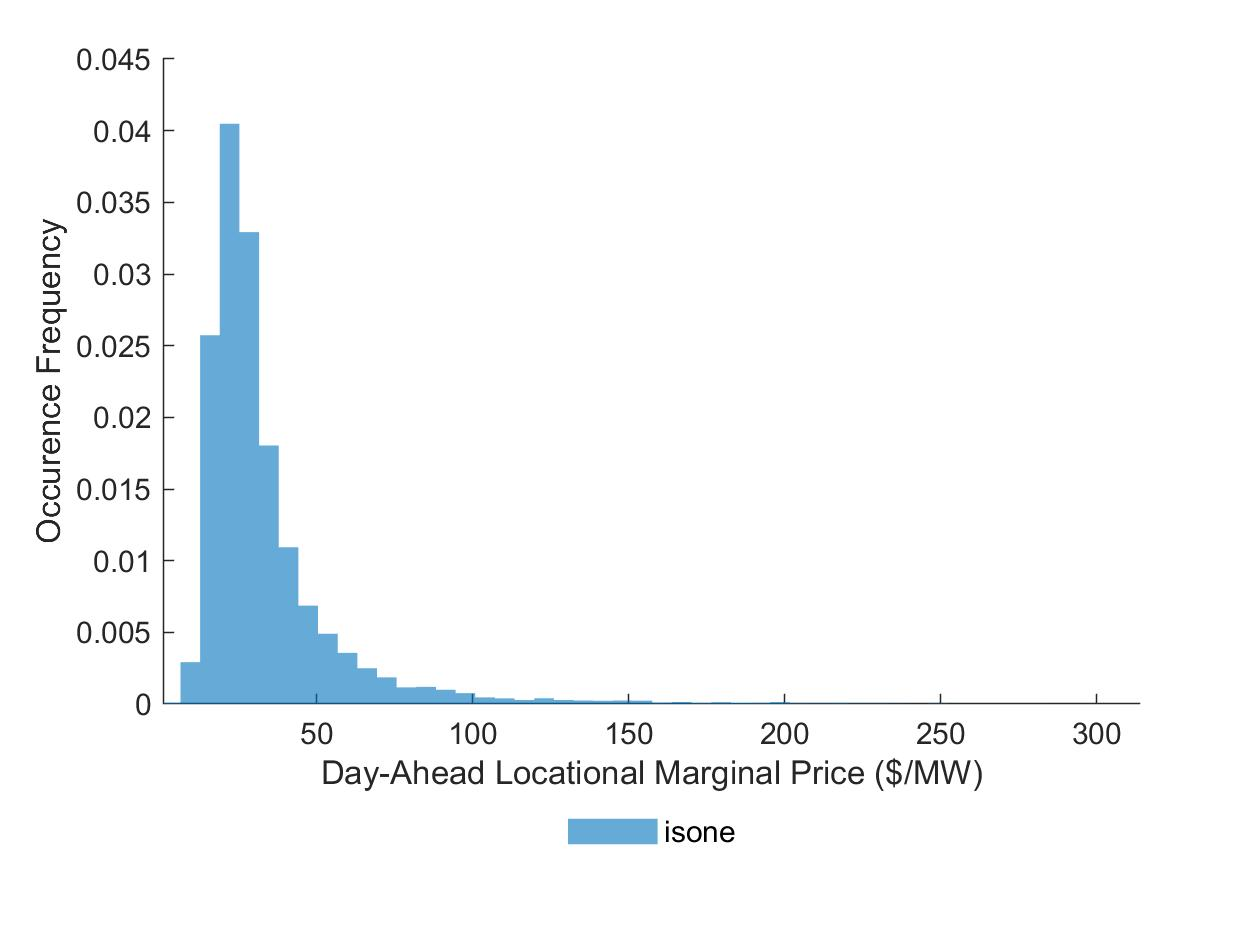
\includegraphics[width=0.8\textwidth]{figures/visualization_example1.jpg}
  \caption{Example: Price Distribution of ISONE} \label{fig:vis_eg1}
\end{figure}

The result is displayed in Figure~\ref{fig:vis_eg1}. By default, the price distribution histogram of ISONE from 2017-01-01 to 2020-07-15 is plotted. If the user wants to change the date range, parameter \verb!DateRange! should be specified. In addition, some of the functions provide an option for resampling data, making them more flexible to use. For example, to plot the average price of every month in 2019, the user may enter

\begin{Command}
 >> plot_price('nyiso','DateRange',{'2019-01-01','2019-12-31'},'ResampleBin'
    ,'month','ResampleMethod','mean');
\end{Command}

\begin{figure}
  \centering
  \noindent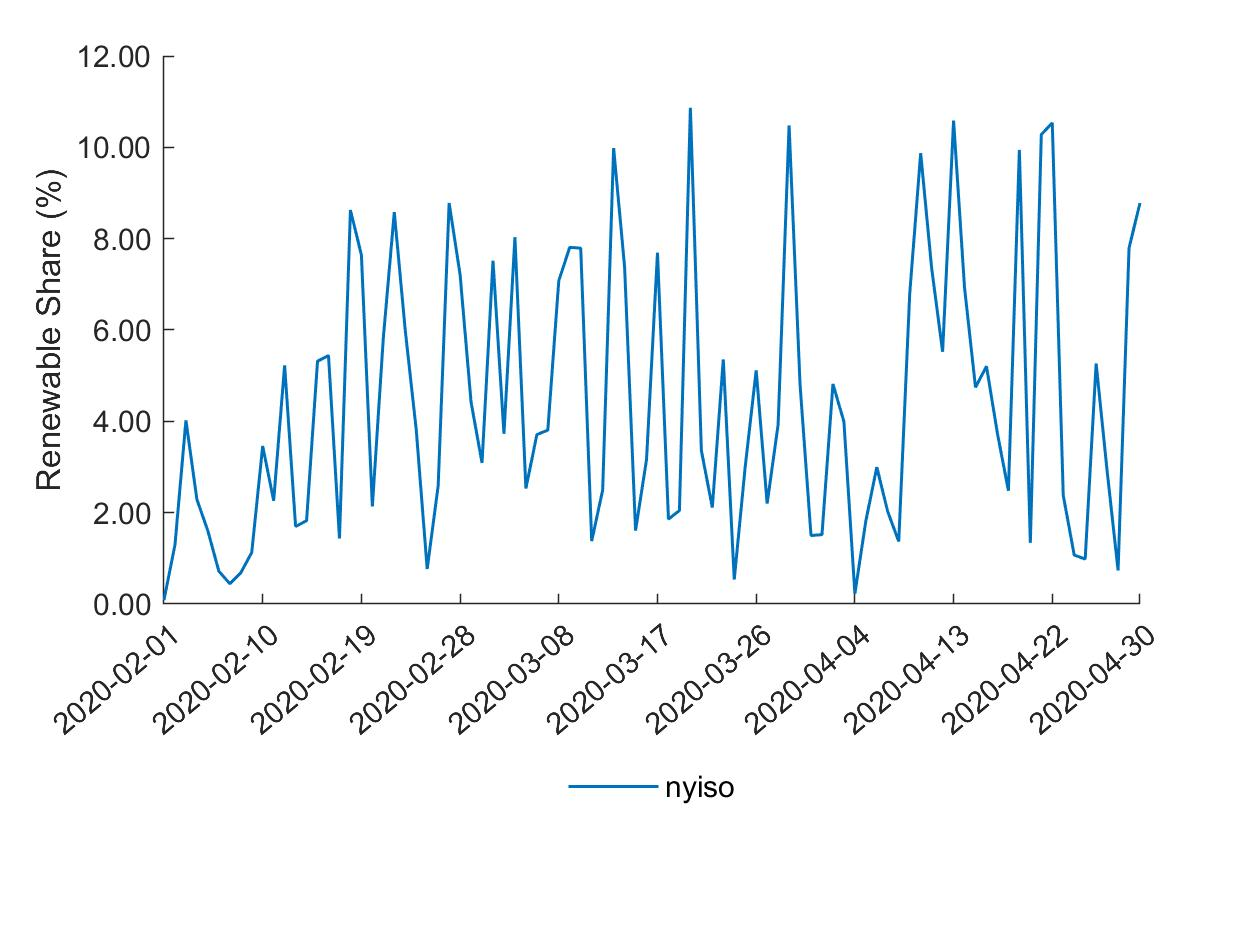
\includegraphics[width=0.8\textwidth]{figures/visualization_example2.jpg}
  \caption{Example: Average Price of NYISO} \label{fig:vis_eg2}
\end{figure}

The result is displayed in Figure~\ref{fig:vis_eg2}, where the desired price trend is plotted.

Like \verb!plot!, all the functions can be used more than once to plot multiple curves in one figure. For example, to plot the demand curves of NYISO in 2018, 2019 and 2020 with date alignment, first calculate the corresponding date range:

\begin{Command}
>> dr_2020=datetime('2020-2-1'):datetime('2020-4-30');
>> dr_2019=dr_2020-calyears(1);
>> dr_2018=dr_2019-calyears(1);
\end{Command}

Thus the desired date ranges for 2018, 2019 and 2020 are \verb!dr_2018!, \verb!dr_2019! and \verb!dr_2020! correspondingly. Now plot the demand curves:

\begin{Command}
>> plot_demand('nyiso','DateRange',dr_2018,'DisplayName','2018','LineStyle',
   ':','Color','#939598');
>> plot_demand('nyiso','DateRange',dr_2019,'DisplayName','2019','LineStyle',
   '--','Color','#D95319');
>> plot_demand('nyiso','DateRange',dr_2020,'DisplayName','2020','Color',
   '#0072BD','LineWidth',2.5);
\end{Command}

\begin{figure}
  \centering
  \noindent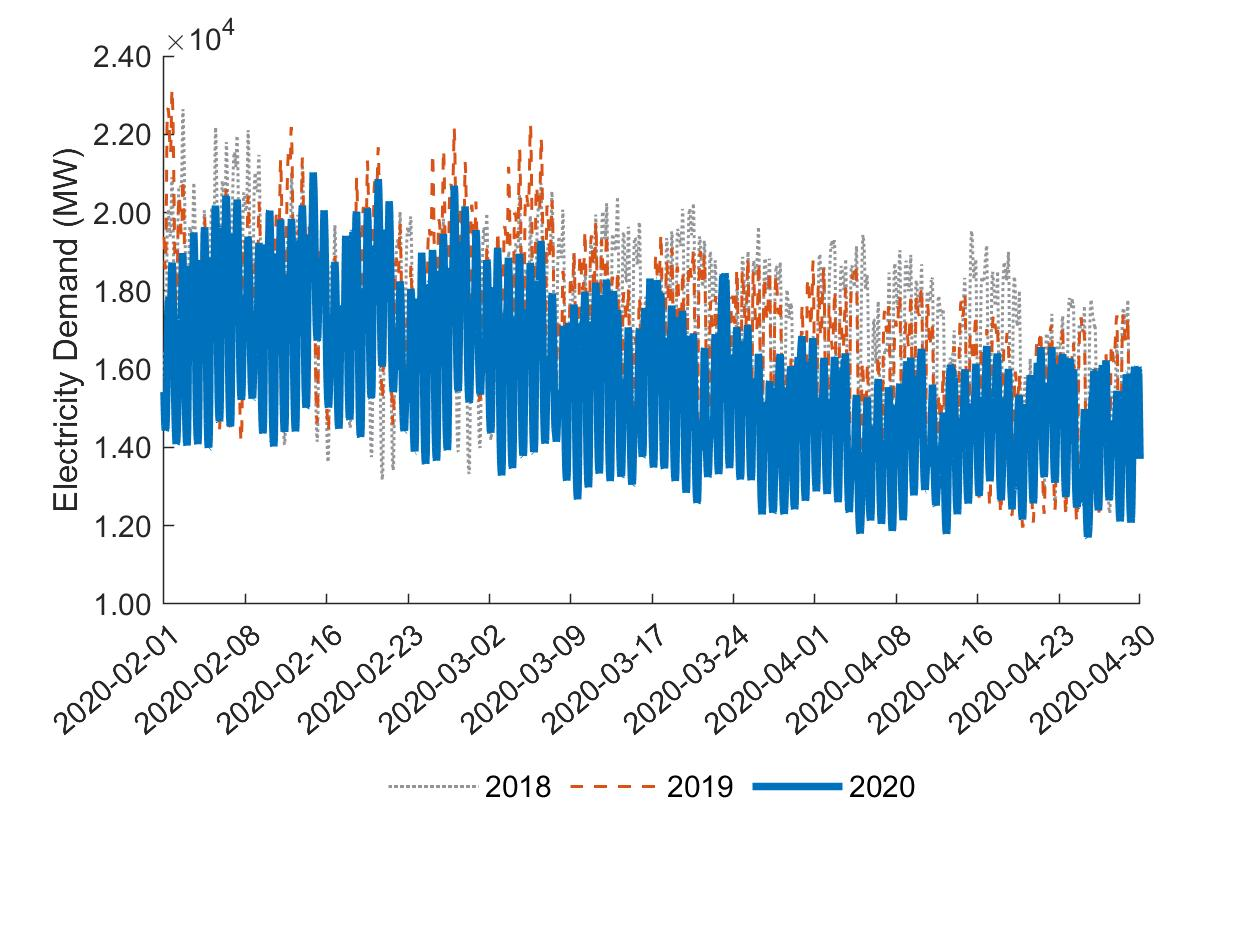
\includegraphics[width=0.8\textwidth]{figures/visualization_example3.jpg}
  \caption{Example: Demand Curves of NYISO} \label{fig:vis_eg3}
\end{figure}

The result is displayed in Figure~\ref{fig:vis_eg3}, where the desired demand curves are plotted. In the example above, several properties of the lines are customized for better recognition. In Section~\ref{subsubsec:vis_cus}, the modification of plots is explored further.



\subsubsection{Customize Plot Properties} \label{subsubsec:vis_cus}

Like \matlab{}, there are mainly two approaches in \covemda{} to modifying a plot: before and after calling the plotting function. The former way refers to passing arguments in the form of \textbf{name-value pairs}, and the latter one refers to changing \textbf{property values} of the chart. They each have their own strengths, and both of them are commonly used to beautify a plot.

In the last example in~\ref{subsubsec:vis_basic}, several properties (label, color and line width) of the three lines are modified by passing name-value pair arguments to the function. In this way, the user is able to integrate multiple modifications in one line of code, making it concise and simple. For example, to display markers at data points, the user may enter

\begin{Command}
>> plot_price('nyiso','DateRange',{'2019-01-01','2019-12-31'},'ResampleBin'
   ,'month','ResampleMethod','mean','Marker','o');
\end{Command}

\begin{figure}
  \centering
  \noindent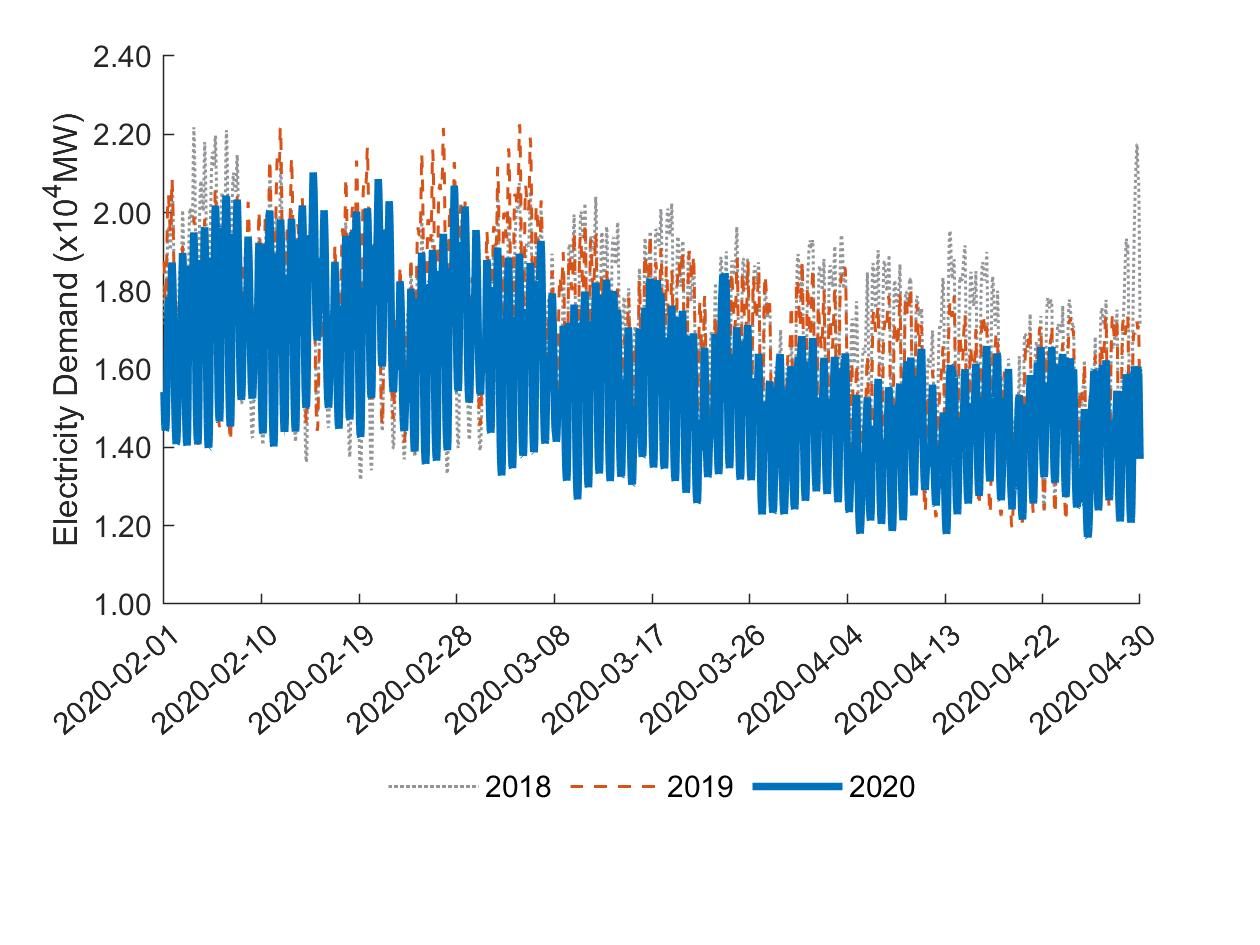
\includegraphics[width=0.8\textwidth]{figures/visualization_example4.jpg}
  \caption{Example: Average Price of NYISO (with Markers)} \label{fig:vis_eg4}
\end{figure}

The result is displayed in Figure~\ref{fig:vis_eg4}, where all the data points are marked with a symbol 'o'. Any other marker symbol can be used in the same way, as long as it is recognized by \verb!plot!.

However, it is difficult to obtain detailed control of the plot by merely passing arguments to the functions, which is why sometimes we also need to change property values after plotting the figure. For example, to change the default display range of y-axis, the user may enter

\begin{Command}
>> plot_daily_demand_curve('nyiso');
>> ax=gca;
>> ax.YLim=[0,4];
\end{Command}

\begin{figure}
  \centering
  \noindent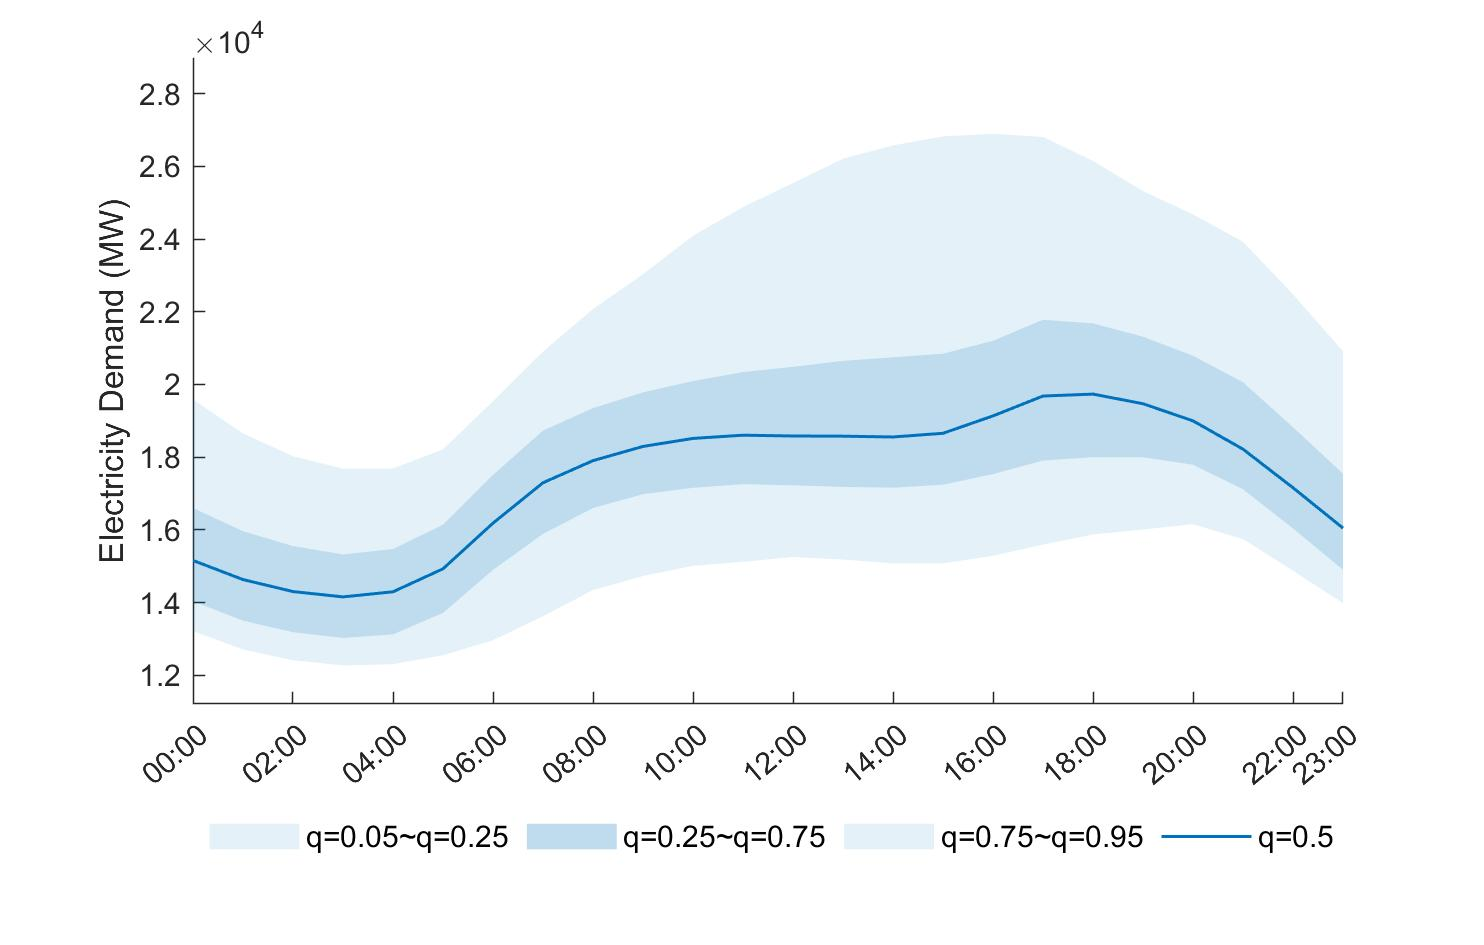
\includegraphics[width=0.8\textwidth]{figures/visualization_example5_1.jpg}
  \caption{Example: Daily Demand Curve of NYISO (Before Changing range of y-axis)} \label{fig:vis_eg5_1}
\end{figure}

\begin{figure}
  \centering
  \noindent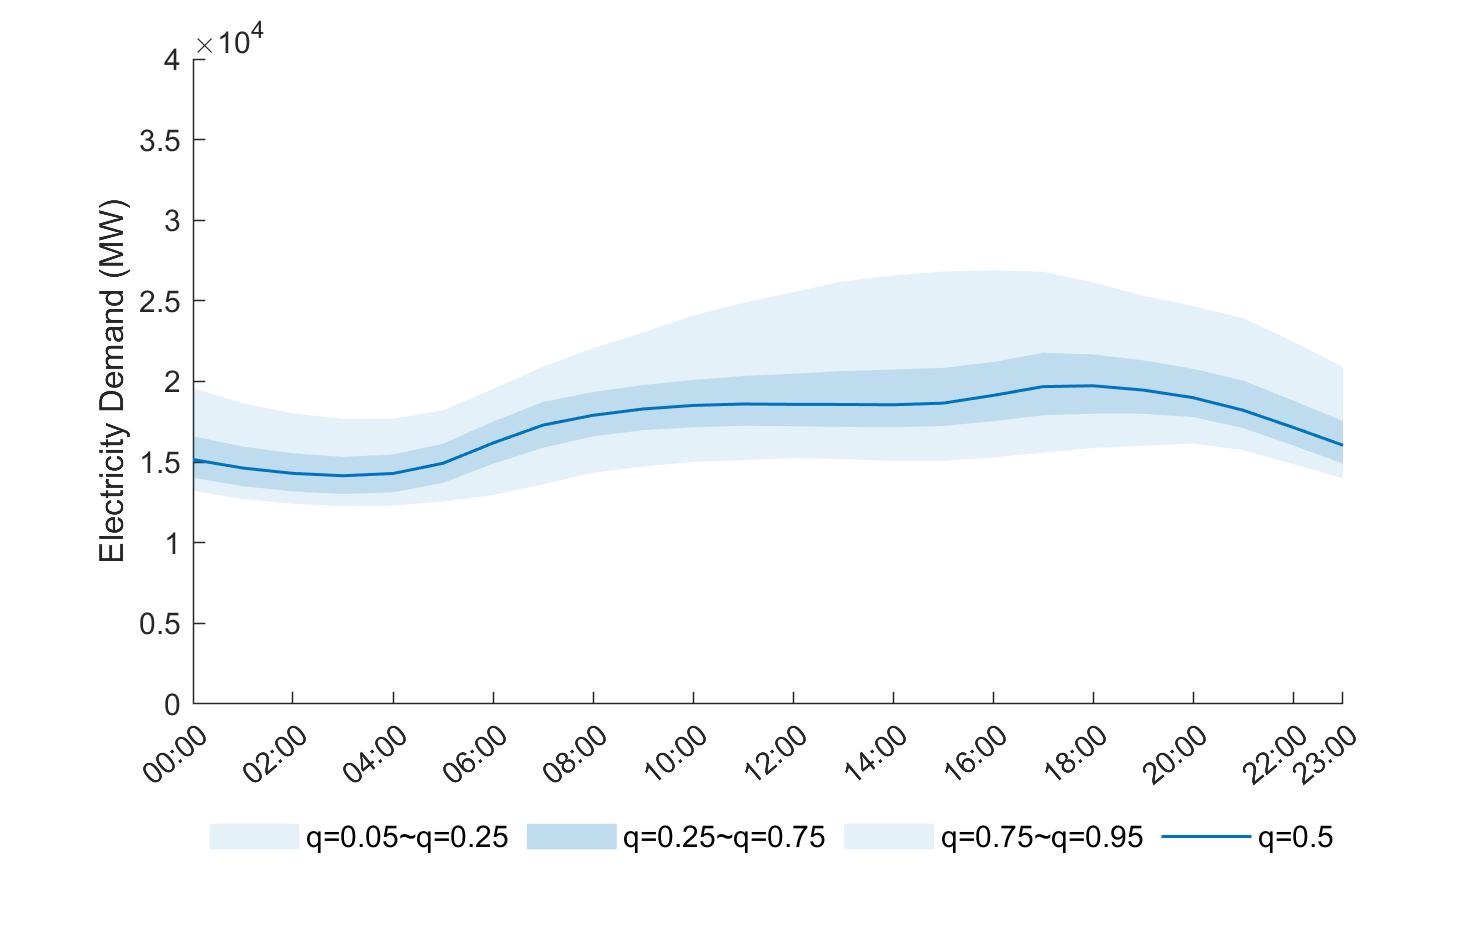
\includegraphics[width=0.8\textwidth]{figures/visualization_example5_2.jpg}
  \caption{Example: Daily Demand Curve of NYISO (After Changing range of y-axis)} \label{fig:vis_eg5_2}
\end{figure}

The result is displayed in Figure~\ref{fig:vis_eg5_1} and~\ref{fig:vis_eg5_2}, where the range of y-axis is enlarged. As the modified property belongs to the axes of the figure rather than area or line objects, the command \verb!ax = gca! is utilized to access the axes. Also, \verb!ylim([0, 4])! (using the function \verb!ylim!) has the same effect as \verb!ax.YLim = [0, 4]! in this case.

Under some circumstances, there may exist more than one object in the graph, which is common when using functions concerning \verb!area!. For example, to highlight renewable energy in a generation mix graph, the user may enter

\begin{Command}
>> ar=plot_generation_mix('spp');
>> ar(1).FaceColor='#868686';
>> ar(2).FaceColor='#acacac';
>> ar(4).FaceColor='#7f7f7f';
>> ar(5).FaceColor='#6b6b6b';
\end{Command}

\begin{figure}
  \centering
  \noindent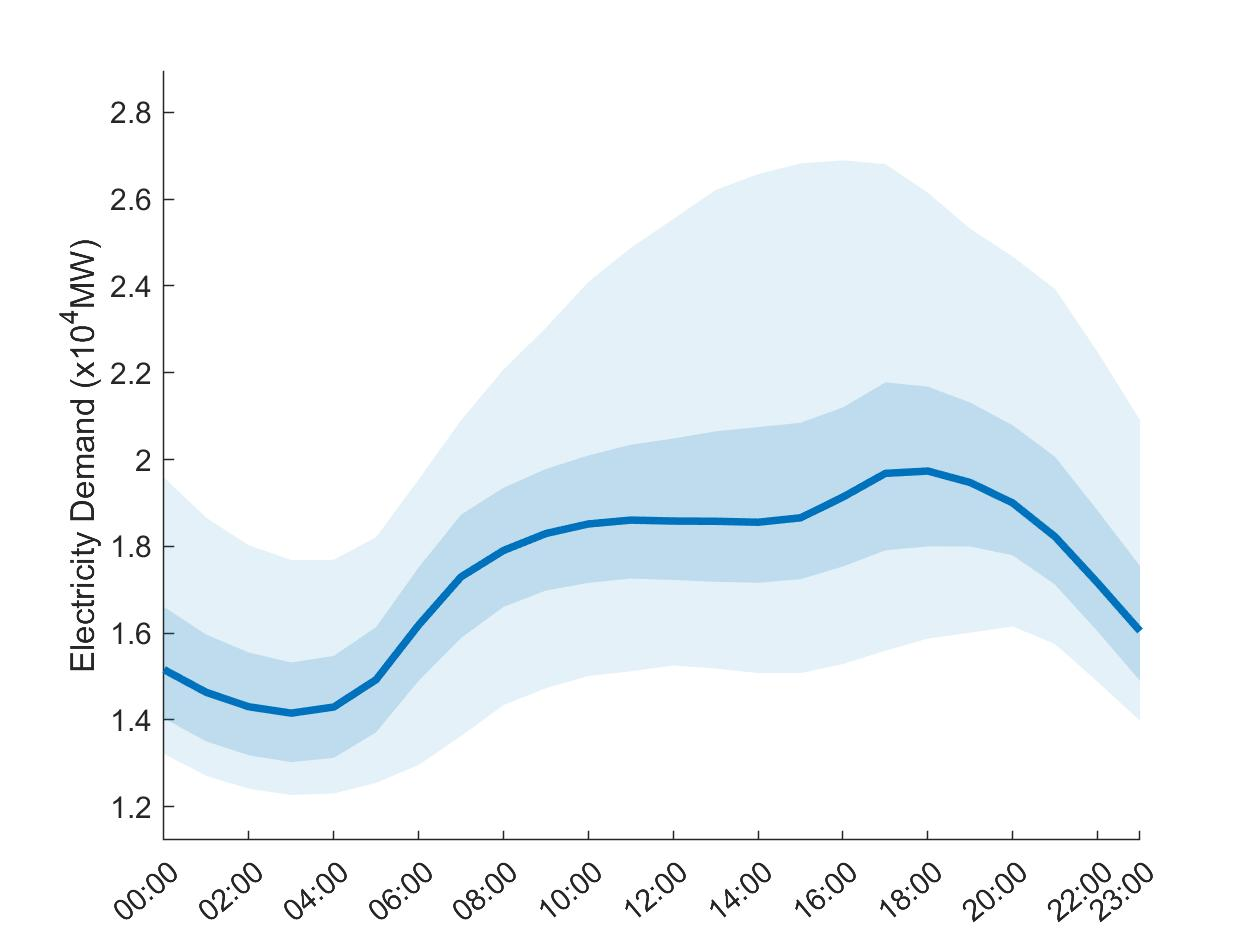
\includegraphics[width=0.8\textwidth]{figures/visualization_example6_1.jpg}
  \caption{Example: Generation Mix of SPP (Before Highlighting Renewables)} \label{fig:vis_eg6_1}
\end{figure}

\begin{figure}
  \centering
  \noindent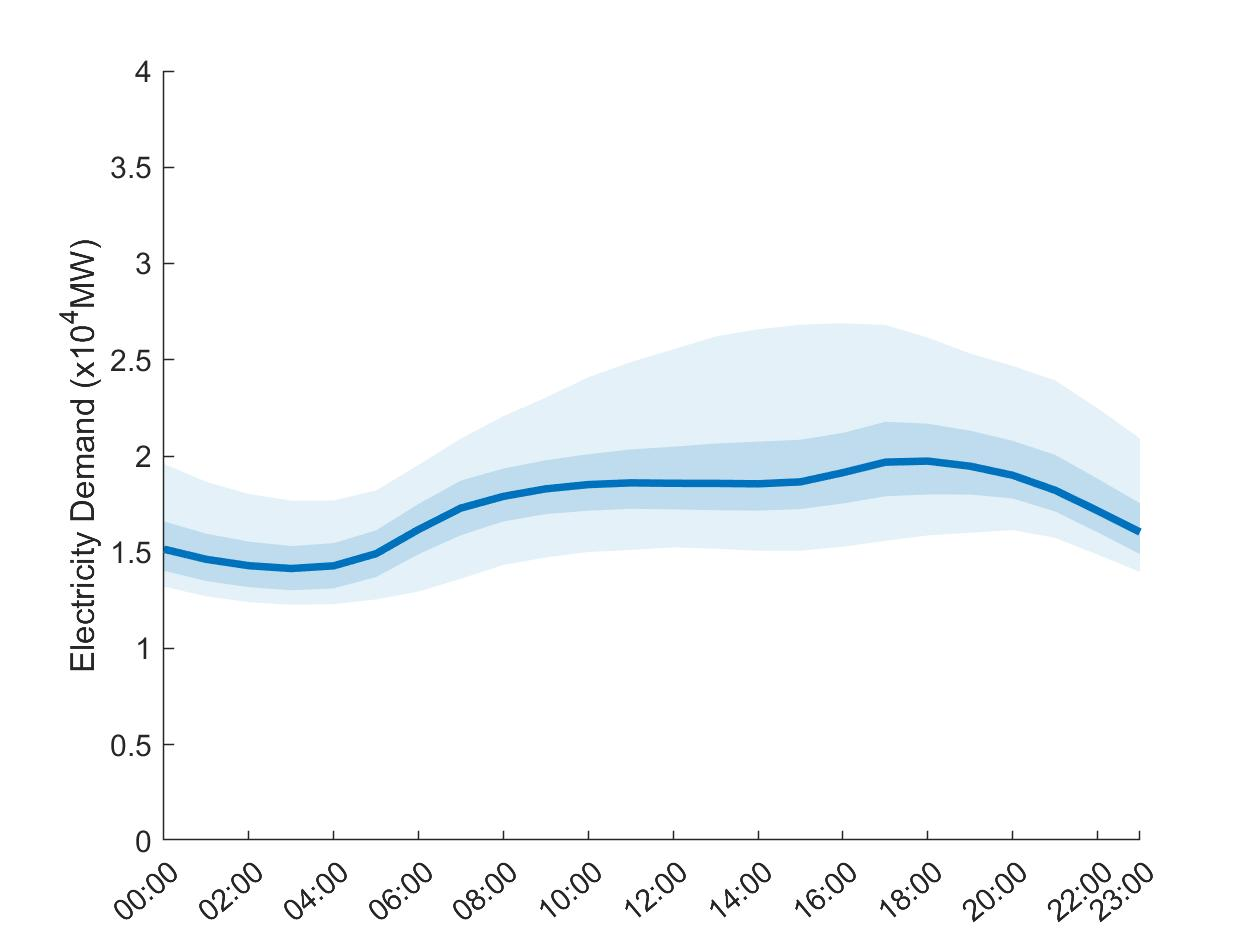
\includegraphics[width=0.8\textwidth]{figures/visualization_example6_2.jpg}
  \caption{Example: Generation Mix of SPP (After Highlighting Renewables)} \label{fig:vis_eg6_2}
\end{figure}

The result is displayed in Figure~\ref{fig:vis_eg6_1} and~\ref{fig:vis_eg6_2}, where the color of all fuel types except hydro, solar and wind are changed to gray after the graph is plotted. Therefore, the renewables are visually highlighted.

Such modifications are obtained by changing property values of certain objects using dot notation. For a list of properties, see \verb!Axes Properties!, \verb!Line Properties!, \verb!Area Properties! and \verb!Histogram Properties!.







%------------------------------------------------
\newpage
\section{Acknowledgments} \label{sec:thanks}

The \covemda{} Project is supported in part by funding from Student Research Training Program of Tsinghua University.

Meanwhile, we would like to acknowledge the professors and judges' suggestions during Tsinghua University Challenge Cup Competition. Thanks to Niklas Kolbe and Mr.Brackets as well.

Last but not least, we are grateful for the support of EI-LAB of Department of Electrical Engineering.







%------------------------------------------------
\begin{appendices}

\newpage
\section{\covemda{}~Files and Functions} \label{sec:}

\subsection{Directory Layout}

\covemda{} root directory contains four folders and two .m files. The two files are \verb!install_covemda.m! and \verb!uninstall_covemda.m! for installation and uninstallation of the toolbox, and folder \verb!high_level!, \verb!low_level! and \verb!basic_operations! contain scripts of all other \covemda{} functions.

Folder \verb!data_temp! contains the temporary files of the toolbox, with two subfolders named \verb!backcast! and \verb!COVID-EMDA!. Folder \verb!COVID-EMDA! contains .csv files obtained from the COVID-EMDA+ data hub, and folder \verb!backcast\supplementary! contains supplementary files for ensemble backcast model (gdp.csv, etc.). Folder \verb!backcast\models! contain pre-trained backcast models and their summary files, sorted in the following format:
\begin{center}
    \verb!models\<market_name>_<city_name_or_rto>\Model_<timestamp>\Models.mat!
    \verb!models\<market_name>_<city_name_or_rto>\Model_<timestamp>\Summary.csv!
\end{center}



\subsection{Functions}  \label{subsec:func_list}

Apart from \verb!install_covemda! and \verb!uninstall_covemda! which are found in the root directory, \covemda{} functions are typically divided into three levels: high level, low level and basic operations, which are also the corresponding folder names. All the high-level and low-level functions are illustrated above at the end of Section~\ref{sec:visual}, Section~\ref{sec:baseline} and Section~\ref{sec:regression}.

\begin{table}[!ht]
    \centering
    \begin{threeparttable}
    \caption{\covemda{} High-level Functions}
    \label{tab:high_level_func}
    \footnotesize
    \begin{tabular}{ll}
        \toprule
        Name & Description \\
        \midrule
        \hyperref[func:cal_abnormal_price_index]{\texttt{cal\_abnormal\_price\_index}} & calculates the abnormal price index in Section~\ref{subsec:abnormal_price_index} \\
        \hyperref[func:cal_baseline]{\texttt{cal\_baseline}} & estimates the load baseline with three methods \\
        \hyperref[func:cal_distribution_diff]{\texttt{cal\_distribution\_diff}} & calculates the Wasserstein difference of price distribution \\
        \hyperref[func:cal_excess_change_rate]{\texttt{cal\_excess\_change\_rate}} & calculates the excess change rate of renewable in Section~\ref{subsec:excess_change_rate} \\
        \hyperref[func:OLS]{\texttt{OLS}} & gives a solution for the OLS regression model in Section~\ref{subsubsec:OLS}\\
        \hyperref[func:VAR]{\texttt{VAR}} & gives a solution for the VAR regression model in Section~\ref{subsubsec:VAR}\\
        \hyperref[func:plot_baseline]{\texttt{plot\_baseline}} & plots the load baseline with different methods \\
        \hyperref[func:plot_daily_demand_curve]{\texttt{plot\_daily\_demand\_curve}} & plots the demand curve with variation in one day \\
        \hyperref[func:plot_demand]{\texttt{plot\_demand}} & plots the demand curve \\
        \hyperref[func:plot_generation_mix]{\texttt{plot\_generation\_mix}} & plots the generation mix \\
        \hyperref[func:plot_mobility]{\texttt{plot\_mobility}} & plots the mobility curve \\
        \hyperref[func:plot_price]{\texttt{plot\_price}} & plots the price curve \\
        \hyperref[func:plot_price_distribution]{\texttt{plot\_price\_distribution}} & plots the price distribution histogram \\
        \hyperref[func:plot_renewable_share]{\texttt{plot\_renewable\_share}} & plots the renewable share curve \\
        \bottomrule
    \end{tabular}
    \end{threeparttable}
\end{table}

\begin{table}[!ht]
    \centering
    \begin{threeparttable}
    \caption{\covemda{} Low-level Functions}
    \label{tab:low_level_func}
    \footnotesize
    \begin{tabular}{ll}
        \toprule
        Name & Description \\
        \midrule
        \hyperref[func:backcast_import_data]{\texttt{backcast\_import\_data}} & imports data for ensemble backcast model \\
        \hyperref[func:backcast_scan_prediction]{\texttt{backcast\_scan\_prediction}} & calculates output of the backcast model for corresponding input \\
        \hyperref[func:backcast_scan_training]{\texttt{backcast\_scan\_training}} & trains the neural networks for the backcast model \\
        \hyperref[func:backcast_test_model]{\texttt{backcast\_test\_model}} & selects the best neural networks to form the backcast model \\
        \hyperref[func:cal_baseline_by_backcast]{\texttt{cal\_baseline\_by\_backcast}} & calculates load baseline by ensemble backcast model \\
        \hyperref[func:cal_baseline_by_dates]{\texttt{cal\_baseline\_by\_dates}} & calculates load baseline by date alignment \\
        \hyperref[func:cal_baseline_by_week_index]{\texttt{cal\_baseline\_by\_week\_index}} & calculates load baseline by week alignment \\
        \hyperref[func:plot_area]{\texttt{plot\_area}} & plots filled areas \\
        \hyperref[func:plot_histogram]{\texttt{plot\_histogram}} & plots histogram \\
        \hyperref[func:plot_line_chart]{\texttt{plot\_line\_chart}} & plots lines \\
        \hyperref[func:plot_quantile]{\texttt{plot\_quantile}} & plots data with variation \\
        \bottomrule
    \end{tabular}
    \end{threeparttable}
\end{table}

\begin{table}[!ht]
    \centering
    \begin{threeparttable}
    \caption{\covemda{} Basic-operation Functions}
    \label{tab:basic_op_func}
    \footnotesize
    \begin{tabular}{ll}
        \toprule
        Name & Description \\
        \midrule
        \verb!basic_backcast_import_models! & imports pre-trained backcast models for baseline estimation \\
        \verb!basic_backcast_save_file! & saves trained models and summary files \\
        \verb!basic_backcast_split_train_and_test! & splits training-validation set and testing set for each backcast model \\
        \verb!basic_backcast_split_train_and_valid! & splits training set and validation set for each network \\
        \verb!basic_backcast_train_and_validate! & trains and validates each network \\
        \verb!basic_calc! & basic four operations for tables \\
        \verb!basic_filter! & applies filter to table \\
        \verb!basic_fitdist! & fits probability distribution for table \\
        \verb!basic_gen_root_dir! & generates the root directory of \covemda{} \\
        \verb!basic_group! & groups the table by non-date columns \\
        \verb!basic_max! & calculates the maximum value of all columns or rows \\
        \verb!basic_mean! & calculates the average value of all columns or rows \\
        \verb!basic_min! & calculates the minimum value of all columns or rows \\
        \verb!basic_plot_preprocess_table! & resamples and groups the table for plotting \\
        \verb!basic_quantile! & calculates the quantile of columns or rows \\
        \verb!basic_read! & reads files from COVID-EMDA+ \\
        \verb!basic_resample! & resamples the table by date \\
        \verb!basic_sum! & sums up all columns or rows \\
        \verb!exchange_column! & exchange two columns in a table\\
        \bottomrule
    \end{tabular}
    \end{threeparttable}
\end{table}

\end{appendices}




\newpage
%\section*{Reference} \label{sec:ref}
%\addcontentsline{toc}{section}{Reference}
\label{sec:ref}

\nocite{rubin2003basic}
\nocite{deeplearninguser}
\nocite{statisticsuser}
\bibliographystyle{IEEEtran}
\bibliography{references}
\end{document}
